\documentclass[12pt, atypical, journal]{article}

\usepackage[utf8]{inputenc}
\usepackage[spanish,es-tabla]{babel}
\usepackage{geometry}
\geometry{letterpaper, margin=2.54cm}
\usepackage{times}
\usepackage{setspace}
\onehalfspacing
\usepackage{graphicx}
\usepackage{booktabs}
\usepackage{longtable}
\usepackage{titlesec}
\usepackage{hyperref}
\usepackage{caption}

\newenvironment{hangparas}[2]{\setlength{\parindent}{-#1}\setlength{\leftmargin}{#1}\everypar{\hangindent=#1}}{\par}

\hypersetup{
   colorlinks=true,
   linkcolor=black,
   filecolor=black,     
   urlcolor=blue,
   citecolor=black
}

\titleformat{\section}{\normalfont\Large\bfseries}{\thesection.}{0.5em}{}
\titleformat{\subsection}{\normalfont\large\bfseries}{\thesubsection.}{0.5em}{}
\titleformat{\subsubsection}{\normalfont\normalsize\bfseries\itshape}{\thesubsubsection.}{0.5em}{}

\usepackage{pgffor}
\usepackage{longtable}
\usepackage{pdfpages}
\usepackage{float}
\usepackage{listings}
\usepackage{xcolor}
\lstset{
    basicstyle=\ttfamily\footnotesize,
    breaklines=true,
    frame=single,
    showstringspaces=false,
    tabsize=2,
    extendedchars=true,
    literate={á}{{\'a}}1 {é}{{\'e}}1 {í}{{\'i}}1 {ó}{{\'o}}1 {ú}{{\'u}}1 {Á}{{\'A}}1 {É}{{\'E}}1 {Í}{{\'I}}1 {Ó}{{\'O}}1 {Ú}{{\'U}}1 {ñ}{{\~n}}1 {Ñ}{{\~N}}1
}

\begin{document}

% ==============================================================================
% 1. PORTADA
% ==============================================================================
\begin{titlepage}
   \begin{center}
       \vspace*{1cm}
      
       {\Large\bfseries UNIVERSIDAD POLITÉCNICA DE CHIAPAS} \\[0.5cm]
       {\large\bfseries INGENIERÍA EN TECNOLOGÍAS DE LA INFORMACIÓN E INNOVACIÓN DIGITAL} \\[1.5cm]
      
       \vfill
      
       {\Large\bfseries REPORTE DE PROYECTO INTEGRADOR II} \\[1cm]
      
       \textbf{Nombre del Proyecto:} \\
       {\large LecturaMétrica: Plataforma Web para la Gestión Automatizada, Analítica y Gamificada del Hábito Lector} \\[1.5cm]
      
       \vfill
      
       \textbf{Integrantes del Equipo:} \\[0.3cm]
       {\large Patricia Alejandra Clemente Chacón (Matrícula: 251237)} \\
       {\large Nínive Argelia Pérez González (Matrícula: 251239)} \\
       {\large Mónica Jamileth Velázquez García (Matrícula: 243729)} \\[1.5cm]
      
       \textbf{Docente:} \\
       {\large Lopez Rojo Viviana} \\[1.5cm]
       
       \textbf{Grado y Grupo:} \\
       {\large 5 B} \\[1.5cm]
      
       \vfill
      
       \textbf{Fecha de entrega:} \\
       {\large 3 de Agosto de 2026}
      
       \vspace*{1cm}
   \end{center}
\end{titlepage}

\newpage

% ==============================================================================
% ÍNDICES
% ==============================================================================
\tableofcontents
\newpage

% ==============================================================================
% 1. Introducción
% ==============================================================================
\section{Introducción}

\subsection{Antecedentes y evidencia}
Las herramientas existentes en el mercado presentan un vacío operativo significativo. Por una parte, existen redes sociales abiertas orientadas a la publicación de textos (como Wattpad o Webtoon) que no ofrecen herramientas métricas personales; por otra parte, plataformas de catálogo literario (como Goodreads) o plantillas de hojas de cálculo (Excel) dependen de un llenado manual repetitivo. Experiencias y estudios de usabilidad en aplicaciones de registro de hábitos demuestran que la alta fricción operativa —es decir, la pérdida de tiempo y el esfuerzo cognitivo que implica registrar datos a mano— es la causa primordial por la cual los usuarios abandonan el uso de estas herramientas durante las primeras semanas, generando frustración e interrumpiendo su ciclo de lectura.

\subsection{Descripción del problema en su contexto}
En la actualidad, muchas personas que desean desarrollar o mantener el hábito de la lectura se enfrentan a la falta de herramientas accesibles para cuantificar su rendimiento diario. En el contexto cotidiano, los lectores se dividen en dos grupos principales que experimentan dificultades similares: por un lado, los lectores principiantes sufren de desmotivación y abandono prematuro al sentir que leer es una actividad aislada y difícil de medir; por otro lado, los lectores habituales —que consumen libros, mangas o novelas gráficas— carecen de un espacio centralizado para organizar grandes volúmenes de capítulos. Al depender de bitácoras manuales o notas dispersas, el control del avance se vuelve una tarea tediosa que termina por interrumpir la constancia del usuario.

\subsection{Objetivo General}
Desarrollar una plataforma web llamada LecturaMétrica que permita optimizar el hábito lector en el público general mediante herramientas de seguimiento automatizado, análisis estadístico multiformato y gestión personalizada de bibliotecas digitales, utilizando un ecosistema tecnológico compuesto por Next.js, Java con Spring Boot y PostgreSQL bajo un modelo de desarrollo híbrido.

\subsection{Objetivos Específicos}
\begin{enumerate}
   \item Diseñar e implementar el módulo de biblioteca personal mediante operaciones CRUD de obras, optimizándolo a través de una arquitectura híbrida de ingesta de datos que combine el consumo de APIs externas de metadatos y rastreadores web para automatizar la extracción de portadas, capítulos y géneros, eliminando la fricción del registro manual.
   \item Desarrollar un componente interactivo de cuantificación de progreso en el \textit{front-end} que ofrezca un flujo dual de captura: un temporizador en tiempo real para la medición automatizada de sesiones activas, y un formulario de registro manual retroactivo para asegurar la flexibilidad de recolección de datos sin importar el entorno del usuario.
   \item Programar la lógica algorítmica para la gestión de un motor de gamificación que procese el cálculo automatizado de rachas consecutivas de días leyendo (\textit{streaks}), récords históricos, asignación de insignias y la inyección automatizada de un ``Radar de Curiosidades'' basado en las preferencias del usuario.
   \item Construir el sistema de mensajería asíncrona ``Buzón del Lector'', implementando las reglas de negocio y filtros necesarios en el servidor para la distribución aleatoria y anónima de micro-reseñas en ciclos controlados de bloqueo y apertura de 24 horas.
   \item Estructurar un \textit{dashboard} analítico dinámico utilizando componentes gráficos interactivos en Next.js para representar la distribución de lectura por géneros literarios, promedios de velocidad lectora real, estimaciones predictivas de finalización de obras y líneas de tiempo de metas cumplidas.
   \item Evaluar el impacto y usabilidad de la plataforma mediante la recolección de datos cuantitativos en una muestra de un mínimo de 40 usuarios reales durante un periodo de 20 días naturales, validando estadísticamente el incremento del tiempo promedio de lectura diario y la tasa de retención activa.
\end{enumerate}

\subsection{Justificación del desarrollo del proyecto}
El desarrollo de \textbf{LecturaMétrica} es fundamental porque ofrece una herramienta que elimina la carga operativa del lector moderno mediante la automatización de datos a través del consumo de servicios externos (como la API de Open Library). Socialmente, aporta una propuesta innovadora para mitigar el aislamiento del lector sin exponerlo a la saturación o toxicidad de las redes sociales tradicionales, lográndolo mediante un intercambio anónimo y controlado de cartas literarias cada 24 horas. Académicamente, el proyecto permite aplicar conceptos avanzados de ingeniería de software, arquitectura web e integración de bases de datos, permitiendo además una evaluación cuantitativa real para medir el incremento del tiempo diario de lectura en un grupo de prueba.

\subsection{Alcances y limitaciones}
El alcance del proyecto contempla el desarrollo de funcionalidades básicas para la gestión de cuentas de usuario, una biblioteca personal para catalogar obras, un temporizador para cronometrar las sesiones de lectura, un tablero de estadísticas y un buzón para intercambiar recomendaciones literarias entre usuarios. Como limitaciones, el sistema no almacena ni visualiza archivos de libros digitales (como PDF o EPUB) por cuestiones de derechos de autor, ni incluye salas de chat públicas en tiempo real.

\subsection{Entregables esperados}
\begin{itemize}
    \item Aplicación Web.
    \item Repositorio Frontend.
    \item Repositorio Backend.
    \item Base de datos funcional.
    \item Documentación técnica.
\end{itemize}

% ==============================================================================
% 2. MARCO REFERENCIAL
% ==============================================================================
\section{Marco Referencial}

\subsection{Marco teórico}
El desarrollo de sistemas de gestión de hábitos de lectura y seguimiento analítico se sustenta en diversos conceptos teóricos y metodológicos provenientes de la ingeniería de software, la psicología conductual y el diseño de sistemas de información. En primer lugar, la arquitectura desacoplada y la Arquitectura Limpia (\textit{Clean Architecture}) propuesta por Robert C. Martin \cite{martin2018} establecen un marco estricto para separar las reglas de negocio de los detalles de infraestructura, frameworks y interfaces de usuario, lo cual garantiza la mantenibilidad y escalabilidad a largo plazo de aplicaciones complejas.

Asimismo, en el ámbito de la psicología cognitiva y la formación de hábitos, las teorías de modificación de conducta sugieren que la reducción de la fricción operativa y la integración de estímulos visuales incrementan significativamente la constancia de los usuarios. En este contexto, la gamificación asíncrona actúa como un mecanismo que, mediante recompensas intermitentes, rachas de lectura (\textit{streaks}) y sistemas de progresión, disminuye la resistencia cognitiva y fomenta la motivación intrínseca sin saturar al usuario con dinámicas sociales invasivas.

\subsection{Estado de la tecnología}

\begin{enumerate}
    \item \textbf{Gestores masivos de bibliotecas (Goodreads, StoryGraph):} Plataformas enfocadas en la catalogación exhaustiva y la reseña literaria. Aunque cuentan con bases de datos inmensas, carecen de herramientas de seguimiento en tiempo real (como temporizadores en web). Además, su principal base de usuarios y diseño nativo se centra en el idioma inglés.
    \item \textbf{Medidores de hábitos y sesiones (Bookmory, Bookly):} Son las herramientas funcionalmente más cercanas al propósito de este proyecto, ya que integran temporizadores, calendarios y estadísticas detalladas. Sin embargo, su enfoque es estrictamente individualista y cerrado, aislando al lector. Aplicaciones como Bookly suelen bloquear funciones hasta pagar una suscripción, mientras que Bookmory carece de mecánicas de interacción comunitaria.
    \item \textbf{Plataformas de autoedición y consumo serializado (Wattpad, Webtoon, Lilithum):} Su núcleo no es la medición del hábito, sino la publicación y el consumo de contenido original. Su componente social es síncrono, directo y a menudo invasivo (comentarios por párrafo o capítulo), lo cual no fomenta la disciplina lectora de obras externas, sino la permanencia dentro de su propio ecosistema de contenido.
\end{enumerate}

A pesar de la popularidad de estas herramientas, el usuario hispanohablante se enfrenta a barreras de idioma o a la falta de una plataforma que equilibre el seguimiento cuantitativo con una motivación comunitaria sana.

\begin{table}[htpb]
\centering
\caption{Análisis comparativo de plataformas de gestión y fomento de lectura}
\label{tab:comparativa_apps}
\resizebox{\textwidth}{!}{
\begin{tabular}{@{}lcccccc@{}}
\toprule
\textbf{Plataforma} & \textbf{Registro por API} & \textbf{Temporizador} & \textbf{Analíticas} & \textbf{Gamificación} & \textbf{Interacción Social} & \textbf{Idioma Nativo} \\
\midrule
\textbf{Goodreads} & Manual / ISBN & No & Básicas & Reto Anual & Foros abiertos & Inglés \\
\textbf{StoryGraph} & Manual / ISBN & No & Avanzadas & Reto Anual & Seguidores & Inglés \\
\textbf{Bookly} & Manual / ISBN & Sí & Avanzadas & Insignias & Nula & Inglés \\
\textbf{Bookmory} & Manual / ISBN & Sí & Avanzadas & Rachas / Calendario & Nula & Multi (Traducido) \\
\textbf{Wattpad / Webtoon / Lilithum} & N/A (Interno) & No & N/A & N/A & Comentarios directos & Español / Multi \\
\midrule
\textbf{LecturaMétrica (Propuesta)} & \textbf{Sí} & \textbf{Sí} & \textbf{Avanzadas} & \textbf{Rachas / Insignias} & \textbf{Buzón Asíncrono} & \textbf{Español} \\
\bottomrule
\end{tabular}
}
\end{table}

Como se observa en la comparativa, \textbf{LecturaMétrica} se posiciona como una solución superior en su nicho al tomar las mejores mecánicas de medición (presentes en aplicaciones como Bookmory) y potenciarlas mediante la inyección de un componente social controlado. El modelo del ``Buzón del Lector'' introduce un intercambio asíncrono y anónimo que genera expectativa y curiosidad sin la presión de las redes sociales tradicionales. Sumado a su arquitectura de ingesta automatizada y su diseño nativo en español, la plataforma elimina la resistencia cognitiva, garantizando una mayor retención del usuario.

\subsection{Contexto tecnológico}
\begin{itemize}
   \item \textbf{Next.js, React y Tailwind CSS, TYpescript:} Framework de desarrollo \textit{front-end} basado en JavaScript y biblioteca de estilos que permite la renderización eficiente de interfaces de usuario basadas en componentes. Su gestión nativa de estados dinámicos combinada con un diseño ágil y adaptable facilita la construcción de gráficos estadísticos interactivos y tableros analíticos en tiempo real.
   \item \textbf{Java y Spring Boot:} Lenguaje de programación fuertemente tipado acoplado a un framework robusto para el desarrollo del \textit{back-end}. Su motor de inversión de control (IoC) e inyección de dependencias permite aislar rígidamente las reglas de negocio del motor de gamificación y la seguridad del servidor.
   \item \textbf{Spring Data JPA e Hibernate:} Tecnologías de mapeo objeto-relacional (ORM) que abstraen la capa de datos en Java, transformando las entidades de software en tablas de bases de datos relacionales y automatizando las consultas transaccionales de alta velocidad.
   \item \textbf{PostgreSQL:} Sistema de gestión de bases de datos relacionales (RDBMS) de código abierto, seleccionado por su alta integridad cuantitativa, soporte avanzado para tipos de datos complejos y eficiencia en el almacenamiento seguro de variables métricas acumuladas.
\end{itemize}

\newpage

% ==============================================================================
% 3. METODOLOGÍA
% ==============================================================================
\section{Metodología}

\subsection{Levantamiento de requerimientos}
El levantamiento de requerimientos para el sistema \textbf{LecturaMétrica} se llevó a cabo mediante la aplicación de técnicas de investigación de campo y análisis documental. Se realizaron entrevistas y cuestionarios preliminares dirigidos a usuarios lectores para identificar las fricciones operativas comunes en el control manual de lecturas, tales como el abandono de bitácoras en papel y la dispersión de información. Asimismo, se examinaron flujos de trabajo de plataformas existentes para determinar las necesidades esenciales que el sistema debía automatizar.

\subsection{Análisis de requerimientos}
A partir de la información recopilada, se procedió al análisis y estructuración de los requerimientos del sistema en dos categorías principales:
\begin{itemize}
    \item \textbf{Requerimientos Funcionales:} Se definieron las capacidades operativas esenciales que la plataforma debe garantizar, tales como el registro e inicio de sesión seguro de usuarios, la gestión del catálogo literario multiformato (libros, mangas, webtoons), la asociación automática de metadatos mediante servicios externos, la actualización incremental de sesiones de lectura y el cálculo automatizado de métricas y rachas de lectura (\textit{streaks}).
    \item \textbf{Requerimientos No Funcionales:} Se establecieron los estándares de calidad, seguridad y rendimiento. Esto incluye cifrado seguro de credenciales mediante BCrypt, protección de rutas y endpoints mediante tokens JWT, alta disponibilidad del servicio y adaptabilidad responsiva de la interfaz de usuario en diversos dispositivos.
\end{itemize}

\subsection{Diseño Base}
El diseño de la solución se estructuró bajo un modelo de arquitectura desacoplada cliente-servidor y un enfoque centrado en el usuario, integrando los siguientes componentes:
\begin{itemize}
    \item \textbf{Historias de Usuario y Modelado Funcional:} Definición de épicas e historias de usuario organizadas por módulos (gestión de biblioteca, sesiones de lectura, perfil, seguridad y buzón asíncrono) para estructurar los requerimientos desde la perspectiva del lector y del administrador.
    \item \textbf{Narrativas de Casos de Uso:} Especificación formal de las interacciones entre los actores y el sistema, documentando flujos normales y alternativos para operaciones críticas como el registro de sesiones de lectura.
    \item \textbf{Prototipos de Interfaces y Maquetado (Figma):} Diseño previo de las pantallas, flujos de navegación y componentes visuales mediante wireframes y prototipos interactivos en Figma, garantizando una experiencia de usuario intuitiva y coherente antes de su codificación.
    \item \textbf{Diagramas del Sistema:} Modelado mediante diagramas de casos de uso UML para delimitar los roles del lector y del administrador, junto con el diagrama Entidad-Relación preliminar y definitivo.
\end{itemize}

\newpage

% ==============================================================================
% 4. ARQUITECTURA ORIENTADA A SERVICIOS (RUBRICA 1)
% ==============================================================================
\section{Arquitectura Orientada a Servicios y Separación de Capas}

\subsection{Arquitectura del ecosistema}
La arquitectura general de \textbf{LecturaMétrica} se fundamenta en un modelo clásico de \textbf{Arquitectura Cliente-Servidor}, evolucionado hacia un enfoque distribuido y desacoplado mediante servicios (API RESTful).

El proyecto se divide físicamente en repositorios independientes para las aplicaciones cliente y el servidor backend. Esta estructura evita el acoplamiento del código, permite un desarrollo modular y facilita la evolución autónoma de cada interfaz. El ecosistema opera bajo cuatro pilares fundamentales:

\begin{itemize}
    \item \textbf{Clientes de Usuario (Capa de Presentación):} Interfaces inteligentes y totalmente independientes del motor de base de datos, gestionan su propio enrutamiento visual y la experiencia de usuario:
    \begin{itemize}
        \item \textit{Aplicación Web Progresiva (PWA):} Aplicación para los lectores finales con adaptabilidad para dispositivos móviles y de escritorio.
        \item \textit{Dashboard de Administración:} Interfaz web simplificada para el personal de gestión.
    \end{itemize}
   
    \item \textbf{Servidor Central (API RESTful):} Núcleo de la lógica de negocio. Es un servicio backend independiente que recibe las peticiones HTTP de los clientes, procesa las reglas del sistema (cálculo de rachas de lectura, validaciones de seguridad y control de sesiones) y devuelve las respuestas en un formato estandarizado. Ningún cliente puede modificar datos sin pasar por la validación de este servidor.
   
    \item \textbf{Capa de Persistencia (Base de Datos):} El almacenamiento transaccional se encuentra aislado en un motor relacional (PostgreSQL). El servidor central es la única entidad autorizada para establecer conexión y ejecutar consultas o modificaciones sobre estas tablas, garantizando la seguridad y la integridad referencial de la información.
   
    \item \textbf{Sistemas y Servicios Externos:} El servidor central y los clientes se integran de manera controlada con herramientas de terceros, tales como la API de \textit{Open Library} para la obtención automática de metadatos literarios e ISBN, y \textit{Cloudinary} para el almacenamiento y optimización en la nube de recursos multimedia (portadas y avatares).
\end{itemize}

\subsection{Diseño de base de datos}
El almacenamiento transaccional de \textbf{LecturaMétrica} está implementado sobre el motor relacional \textbf{PostgreSQL}. El esquema fue diseñado bajo la tercera forma normal (3NF) para evitar la redundancia de datos y garantizar la integridad referencial a través de restricciones de llave foránea (\textit{Foreign Keys}).

\subsubsection{Decisiones estratégicas de diseño}
El modelado de la base de datos incorpora tres patrones arquitectónicos clave para optimizar la seguridad, el rendimiento y la trazabilidad del sistema:
\begin{itemize}
    \item \textbf{Estrategia híbrida de identificadores:} Las entidades transaccionales y de usuario (\texttt{users}, \texttt{books}, \texttt{user\_library}, \texttt{reading\_sessions}) utilizan identificadores únicos universales (\textbf{UUID}). Esto previene ataques de enumeración en la API y facilita la escalabilidad horizontal. Por otro lado, los catálogos y diccionarios (\texttt{authors}, \texttt{genders}, \texttt{formats}, \texttt{badges}) emplean enteros largos autoincrementables (\textbf{BIGINT}), optimizando el indexado y la velocidad de las consultas relacionales más frecuentes.
    \item \textbf{Trazabilidad y Borrado Suave (\textit{Soft Delete}):} Entidades principales como usuarios, libros, autores y estados integran banderas booleanas (\texttt{deleted}) y marcas de tiempo (\texttt{deleted\_at}). Esto permite desactivar registros en la lógica de negocio sin destruirlos físicamente, preservando la coherencia de las estadísticas e historiales de lectura.
    \item \textbf{Auditoría temporal:} La mayoría de las tablas incorporan atributos de control de tiempo (\texttt{created\_at}, \texttt{updated\_at}) para registrar el ciclo de vida de la información sin depender de bitácoras externas.
\end{itemize}

\subsubsection{Estructura relacional por dominios de negocio}
Para facilitar su comprensión y mantenimiento, el esquema de 22 tablas se agrupa en cinco dominios funcionales que reflejan directamente los módulos del backend:

\begin{table}[H]
\centering
\footnotesize
\begin{tabular}{|p{3.5cm}|p{2.3cm}|p{2cm}|p{5.5cm}|}
\hline
\textbf{Tabla} & \textbf{Llave Primaria} & \textbf{Tipo de Dato} & \textbf{Descripción y Responsabilidad} \\ \hline
\texttt{users} & \texttt{id} & \texttt{UUID} & Credenciales, metas anuales de lectura y relación con rol y fotografía. \\ \hline
\texttt{roles} & \texttt{id} & \texttt{UUID} & Catálogo de roles de acceso al sistema (Ej. Lector, Administrador). \\ \hline
\texttt{pictures} & \texttt{id} & \texttt{BIGINT} & Almacenamiento y URL de avatares sincronizados con Cloudinary. \\ \hline
\end{tabular}
\caption{Dominio 1: Gestión de Usuarios y Seguridad.}
\label{tab:db_users}
\end{table}

\begin{table}[H]
\centering
\footnotesize
\begin{tabular}{|p{3.5cm}|p{2.3cm}|p{2cm}|p{5.5cm}|}
\hline
\textbf{Tabla} & \textbf{Llave Primaria} & \textbf{Tipo de Dato} & \textbf{Descripción y Responsabilidad} \\ \hline
\texttt{books} & \texttt{id} & \texttt{UUID} & Catálogo central de obras literarias, código ISBN y URL de portada. \\ \hline
\texttt{authors} & \texttt{id} & \texttt{BIGINT} & Registro de autores literarios con soporte de borrado suave. \\ \hline
\texttt{genders} & \texttt{id} & \texttt{BIGINT} & Catálogo de géneros y clasificaciones literarias. \\ \hline
\texttt{formats} & \texttt{id} & \texttt{BIGINT} & Tipos de formato de lectura (Físico, Digital, Audiolibro). \\ \hline
\texttt{book\_authors} & \texttt{book\_id, author\_id} & \texttt{UUID / BIGINT} & Tabla intermedia para la relación N:M entre obras y autores. \\ \hline
\texttt{book\_genres} & \texttt{book\_id, gender\_id} & \texttt{UUID / BIGINT} & Tabla intermedia para la relación N:M entre obras y géneros. \\ \hline
\end{tabular}
\caption{Dominio 2: Catálogo Literario y Clasificación.}
\label{tab:db_books}
\end{table}

\begin{table}[H]
\centering
\footnotesize
\begin{tabular}{|p{3.5cm}|p{2.3cm}|p{2cm}|p{5.5cm}|}
\hline
\textbf{Tabla} & \textbf{Llave Primaria} & \textbf{Tipo de Dato} & \textbf{Descripción y Responsabilidad} \\ \hline
\texttt{user\_library} & \texttt{id} & \texttt{UUID} & Biblioteca personal del usuario, progreso actual y libro favorito. \\ \hline
\texttt{reading\_status} & \texttt{id} & \texttt{BIGINT} & Catálogo de estados de lectura (Por leer, Leyendo, Terminado). \\ \hline
\texttt{reading\_sessions}& \texttt{id} & \texttt{UUID} & Historial de lecturas con registro exacto de segundos, páginas y capítulos. \\ \hline
\texttt{library\_notes} & \texttt{id} & \texttt{BIGINT} & Notas y reflexiones guardadas por el usuario por página o capítulo. \\ \hline
\end{tabular}
\caption{Dominio 3: Biblioteca Personal, Sesiones y Notas.}
\label{tab:db_library}
\end{table}

\begin{table}[H]
\centering
\footnotesize
\begin{tabular}{|p{3.5cm}|p{2.3cm}|p{2cm}|p{5.5cm}|}
\hline
\textbf{Tabla} & \textbf{Llave Primaria} & \textbf{Tipo de Dato} & \textbf{Descripción y Responsabilidad} \\ \hline
\texttt{user\_streaks} & \texttt{id} & \texttt{UUID} & Control de racha actual, racha máxima y última fecha de actividad. \\ \hline
\texttt{badges} & \texttt{id} & \texttt{BIGINT} & Catálogo de insignias y recompensas visuales de la plataforma. \\ \hline
\texttt{user\_badges} & \texttt{id} & \texttt{BIGINT} & Registro de insignias y logros desbloqueados por cada usuario. \\ \hline
\texttt{curiosities} & \texttt{id} & \texttt{BIGINT} & Datos curiosos aleatorios para el radar de descubrimiento. \\ \hline
\end{tabular}
\caption{Dominio 4: Gamificación, Rachas y Descubrimiento.}
\label{tab:db_gamification}
\end{table}

\begin{table}[H]
\centering
\footnotesize
\begin{tabular}{|p{3.7cm}|p{2.1cm}|p{2cm}|p{5.5cm}|}
\hline
\textbf{Tabla} & \textbf{Llave Primaria} & \textbf{Tipo de Dato} & \textbf{Descripción y Responsabilidad} \\ \hline
\texttt{recommendations} & \texttt{id} & \texttt{UUID} & Perfil general de preferencias y configuración del lector. \\ \hline
\texttt{user\_pref\_formats} & \texttt{pref\_id, formats\_id} & \texttt{UUID / BIGINT} & Tabla intermedia que enlaza al usuario con sus formatos preferidos. \\ \hline
\texttt{user\_pref\_genres} & \texttt{pref\_id, genres\_id} & \texttt{UUID / BIGINT} & Tabla intermedia que enlaza al usuario con sus géneros preferidos. \\ \hline
\texttt{recommendation\_contents} & \texttt{id} & \texttt{BIGINT} & Contenido literario y mensajes para las recomendaciones creadas. \\ \hline
\texttt{letters} & \texttt{id} & \texttt{BIGINT} & Buzón de cartas para intercambio asíncrono y reclamo de lecturas. \\ \hline
\end{tabular}
\caption{Dominio 5: Recomendaciones y Buzón de Cartas.}
\label{tab:db_social}
\end{table}

\begin{figure}[H]
    \centering
    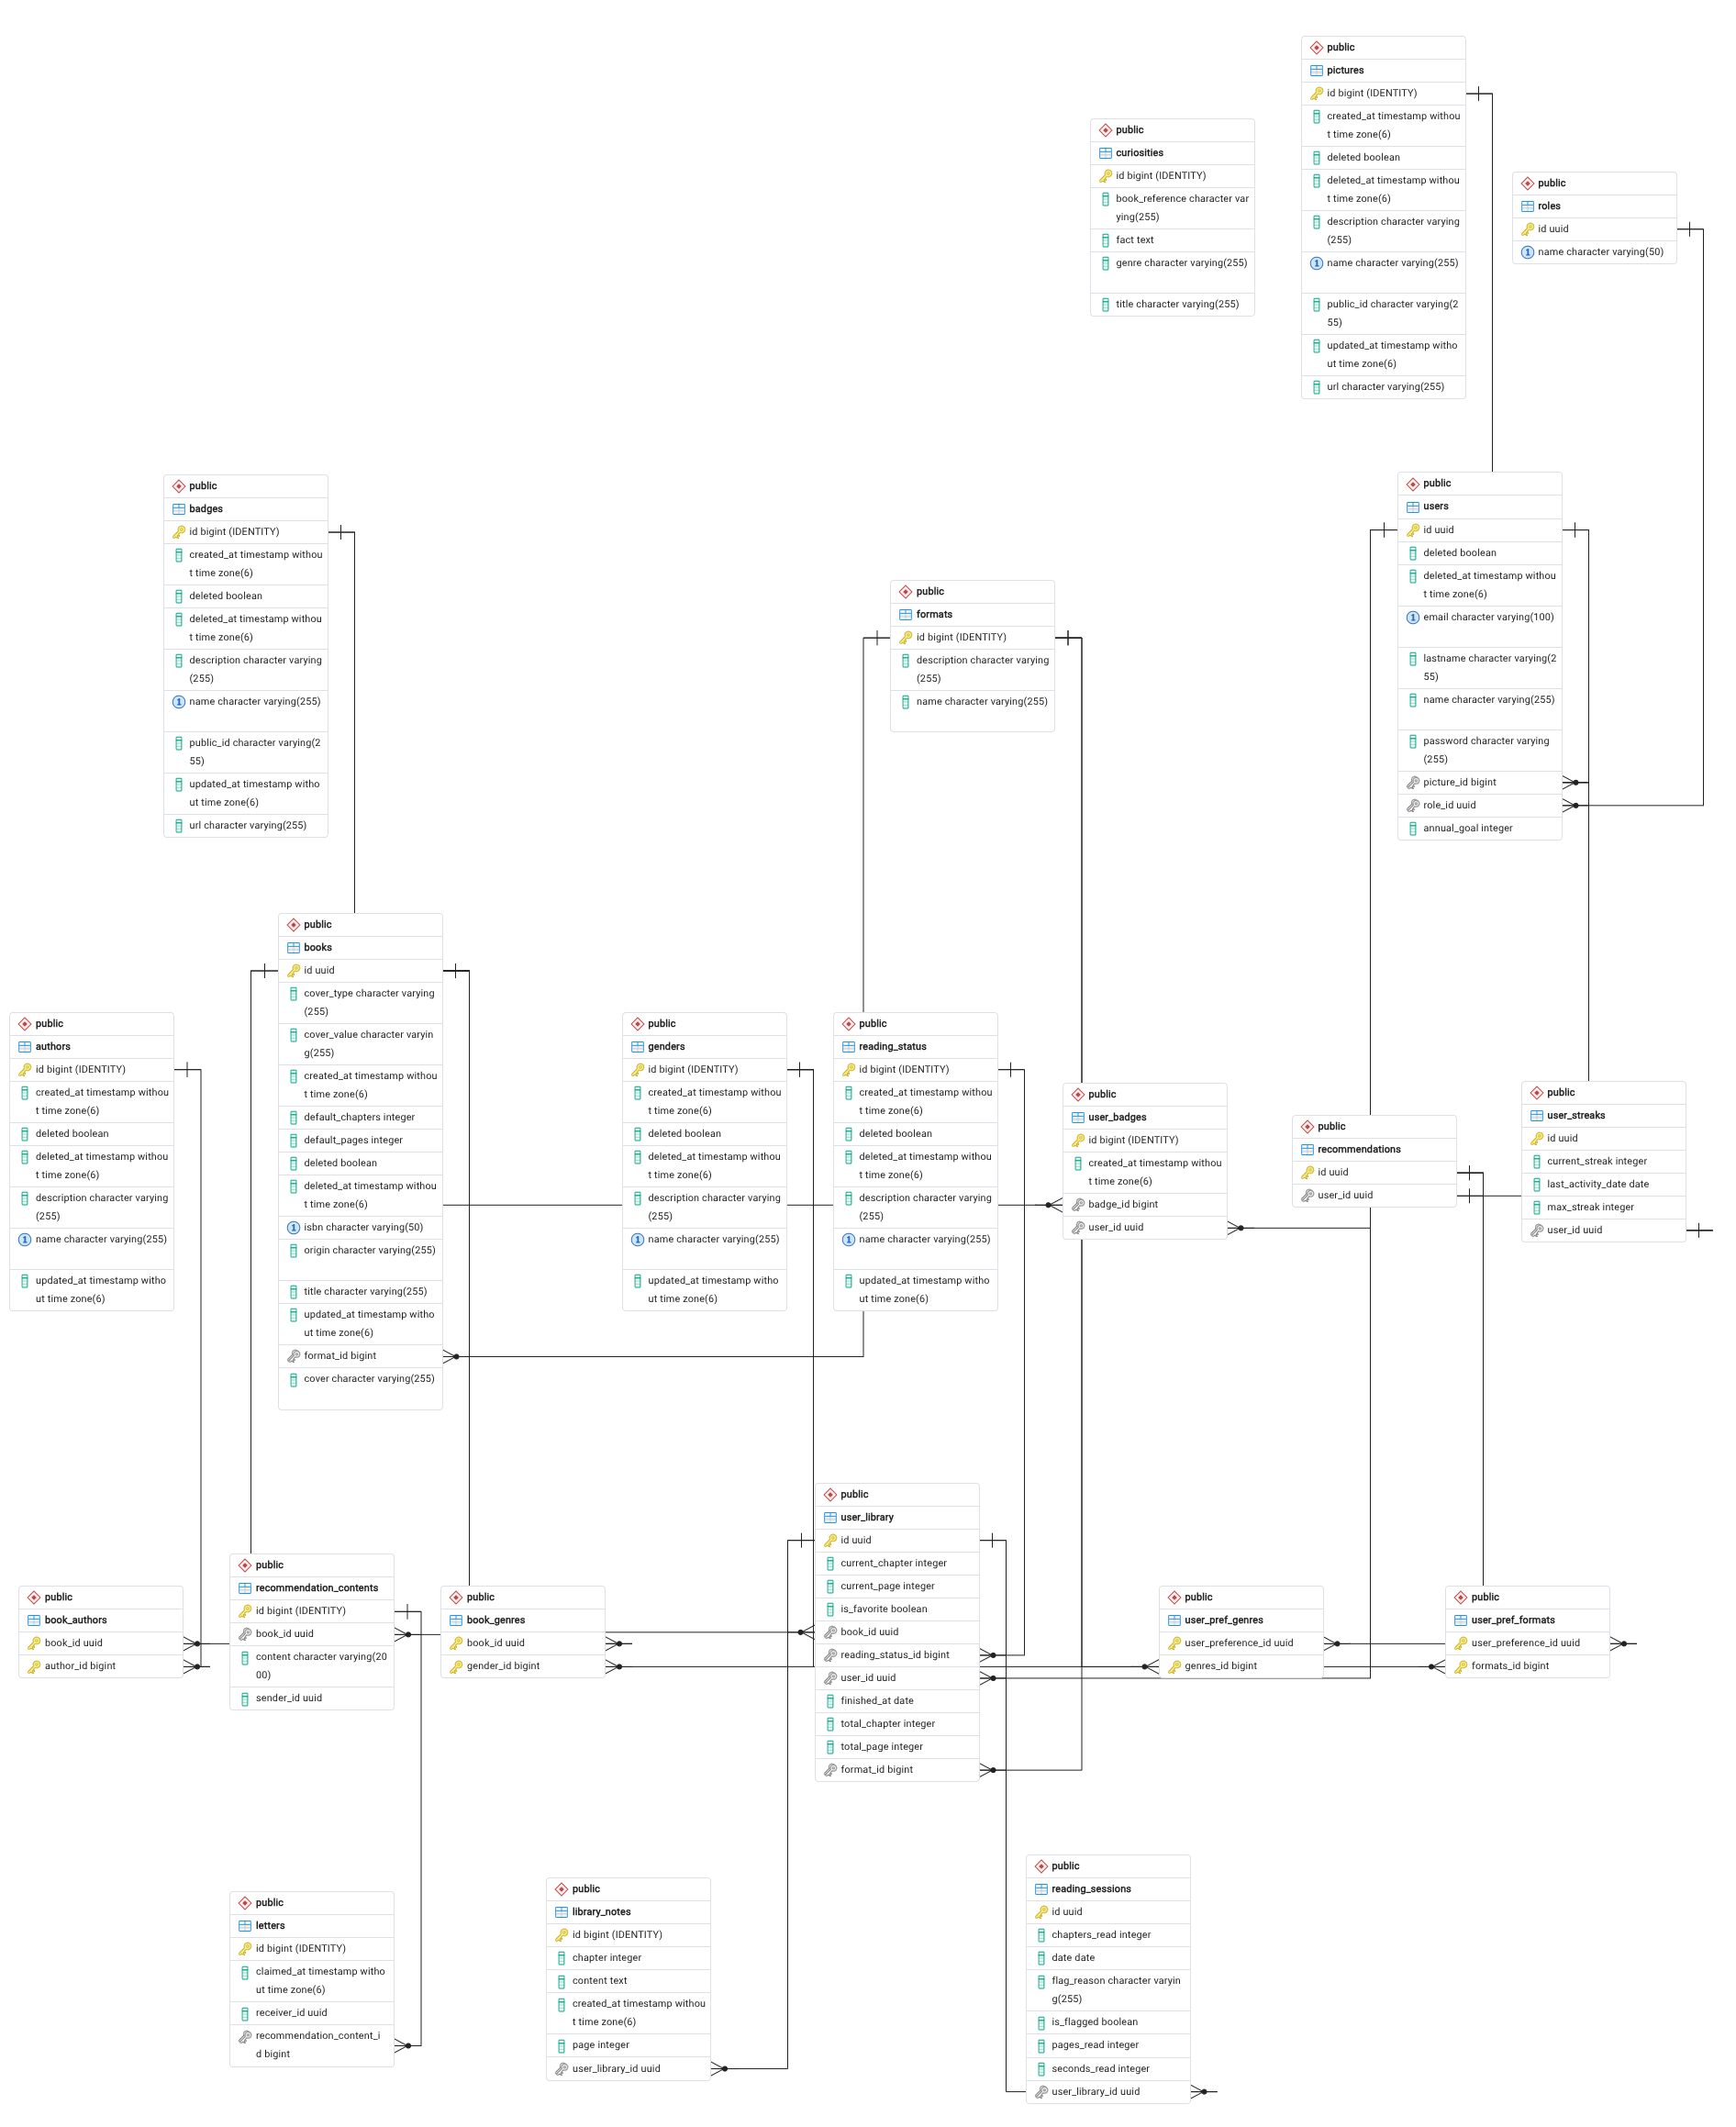
\includegraphics[width=0.9\textwidth]{./fotos/code/database.png}
    \caption{Diagrama Entidad-Relación de LecturaMétrica.}
    \label{fig:database}
\end{figure}

\subsubsection{Diccionario de datos y especificación técnica de columnas}
Para garantizar la integridad referencial y estandarizar el desarrollo entre el equipo de backend y base de datos, cada entidad del modelo relacional cuenta con una especificación estricta de tipos de datos, restricciones de nulidad y llaves de índice. 

A continuación, se presenta como muestra representativa la estructura técnica de la entidad central del negocio (\texttt{user\_library}), la cual gestiona la relación entre el lector y las obras de su catálogo personal:

\begin{table}[H]
    \centering
    \footnotesize
    \begin{tabular}{|l|l|c|p{6.5cm}|}
        \hline
        \textbf{Atributo} & \textbf{Tipo de Dato} & \textbf{Llave} & \textbf{Descripción y Restricción} \\ \hline
        \texttt{id} & \texttt{UUID} & PK & Identificador único e irrepetible del registro en la biblioteca. \\ \hline
        \texttt{user\_id} & \texttt{UUID} & FK & Referencia al propietario de la biblioteca \texttt{users(id)}. \\ \hline
        \texttt{book\_id} & \texttt{UUID} & FK & Referencia a la obra literaria \texttt{books(id)}. \\ \hline
        \texttt{format\_id} & \texttt{BIGINT} & FK & Referencia al formato de lectura \texttt{formats(id)}. \\ \hline
        \texttt{reading\_status\_id} & \texttt{BIGINT} & FK & Referencia al estado de lectura \texttt{reading\_status(id)}. \\ \hline
        \texttt{current\_page} & \texttt{INTEGER} & - & Página actual de avance ($0 \le \mathrm{valor} \le \mathrm{total\_page}$). \\ \hline
        \texttt{total\_page} & \texttt{INTEGER} & - & Total de páginas de la obra. \\ \hline
        \texttt{current\_chapter} & \texttt{INTEGER} & - & Capítulo actual de avance. \\ \hline
        \texttt{total\_chapter} & \texttt{INTEGER} & - & Total de capítulos de la obra. \\ \hline
        \texttt{is\_favorite} & \texttt{BOOLEAN} & - & Indicador booleano de obra favorita (por defecto \texttt{false}). \\ \hline
        \texttt{finished\_at} & \texttt{DATE} & - & Fecha en que el usuario completó la lectura (nulo si sigue leyendo). \\ \hline
    \end{tabular}
    \caption{Especificación técnica de columnas para la entidad \texttt{user\_library}.}
    \label{tab:sample_data_dictionary}
\end{table}

\vspace{0.2cm}
\begin{quote}
\textit{\textbf{Nota aclaratoria:} La tabla anterior (\ref{tab:sample_data_dictionary}) ilustra el estándar de modelado y tipado utilizado para la especificación física de la base de datos en PostgreSQL. Por cuestiones de legibilidad y para mantener la fluidez del presente documento técnico, el diccionario de datos exhaustivo con las especificaciones de las 22 tablas del sistema (incluyendo catálogos, tablas pivote $N:M$ y entidades de gamificación) se adjunta para su consulta integral en el \textbf{Anexo C: Diccionario de Datos del Sistema Relacional}.}
\end{quote}

\newpage

% ==============================================================================
% 5. IMPLEMENTACIÓN TÉCNICA BACKEND (RUBRICA 2)
% ==============================================================================
\section{Implementación Técnica del Backend y Diseño de API}

\subsection{Diseño del backend y Arquitectura Limpia}
El diseño del servidor de \textbf{LecturaMétrica} se fundamenta en los principios de la Arquitectura Limpia (\textit{Clean Architecture}). Esta decisión arquitectónica se tomó para desacoplar completamente la lógica central del negocio de las dependencias externas (como bases de datos, frameworks web y servicios de terceros), garantizando así un sistema escalable, mantenible y altamente testeable

El desarrollo se implementó en \textbf{Java 21} utilizando el ecosistema de \textbf{Spring Boot}, lo que facilita la inyección de dependencias y el mapeo objeto-relacional (ORM) a través de Spring Data JPA e Hibernate. 
Todo el código está organizado bajo un enfoque modular por características (\textit{Feature-driven structure}), donde cada dominio principal (como libros, usuarios, biblioteca, rachas y buzón) se encapsula de forma independiente.

\subsection{Estructura de capas por módulo}
Para asegurar la separación de responsabilidades, cada módulo dentro del sistema se subdivide estrictamente en tres capas lógicas.

\begin{enumerate}
    \item \textbf{Capa de Dominio:} Es el núcleo de la aplicación. Contiene las entidades (modelos de datos puros) y los eventos del dominio. Esta capa no tiene ninguna dependencia hacia Spring Boot u otras bibliotecas externas, asegurando que las reglas de negocio permanezcan puras.
   
    \item \textbf{Capa de Aplicación:} Contiene los casos de uso (\textit{Use Cases}) que orquestan la lógica del negocio. Ejemplos de esto son los servicios encargados de registrar nuevas obras, actualizar las rachas diarias de lectura o calcular el radar de preferencias del usuario.
   
    \item \textbf{Capa de Infraestructura (\textit{Infrastructure Layer}):} Es la capa más externa y se encarga de los detalles de implementación, se encuentran: 
    \begin{itemize}
        \item \textbf{Controladores REST (\textit{Routing/Controllers}):} Manejan las peticiones HTTP y exponen los \textit{endpoints} de comunicación.
        \item \textbf{Data Transfer Objects (DTOs) y Mapeadores:} Se aseguran de que las propiedades crudas de las peticiones no interactúen directamente con la capa de aplicación. Transforman los datos de entrada a modelos de dominio antes de ser procesados.
        \item \textbf{Repositorios:} Interfaces que gestionan la conexión directa con la base de datos PostgreSQL.
        \item \textbf{Clientes Externos (\textit{Clients}):} Adaptadores para comunicarse con APIs externas, utilizados principalmente para la ingesta de metadatos de los libros.
    \end{itemize}
\end{enumerate}

\subsection{Lógica de Negocio y Fragmentos de Código Clave (Backend)}

\subsubsection{Consumo de API Externa (\texttt{OpenLibraryClient})}
El cliente gestiona la petición HTTP a la API de Open Library y procesa la respuesta mediante registros internos para extraer los metadatos esenciales de forma eficiente:

\begin{lstlisting}[language=Java, basicstyle=\ttfamily\footnotesize, breaklines=true, frame=single]
@Override
public List<CreateBookRequest> searchExternalBooks(String query) {
    String url = "https://openlibrary.org/search.json?q=" + query +
            "&limit=5&fields=title,author_name,isbn,subject,cover_i";
    List<CreateBookRequest> results = new ArrayList<>();
   
    try {
        var response = restTemplate.getForObject(url, OpenLibraryResponse.class);
        if (response != null && response.docs() != null) {
            for (Doc info : response.docs()) {
                String isbn = (info.isbn() != null && !info.isbn().isEmpty())
                        ? info.isbn().get(0) : "EXT-" + UUID.randomUUID().toString().substring(0, 8);
               
                String cover = info.cover_i() != null ?
                        "https://covers.openlibrary.org/b/id/" + info.cover_i() + "-M.jpg" : null;

                results.add(new CreateBookRequest(isbn, info.title(), null, null, cover));
            }
        }
    } catch (Exception e) {
        System.err.println("Error al consumir OpenLibrary API: " + e.getMessage());
    }
    return results;
}
\end{lstlisting}

\subsubsection{Control y Actualización de Rachas (\texttt{UpdateUserStreakUseCase})}
Este algoritmo compara la fecha actual con la última actividad registrada para incrementar o reiniciar de forma atómica la racha de lectura del usuario:

\begin{lstlisting}[language=Java, basicstyle=\ttfamily\footnotesize, breaklines=true, frame=single]
@Transactional(propagation = Propagation.REQUIRES_NEW)
public void execute(UUID userId) {
    LocalDate today = dateProvider.getToday();
    UserStreak streak = userStreakRepository.findByUserId(userId)
            .orElseGet(() -> createInitialStreak(userId));

    if (streak.getLastActivityDate() == null) {
        streak.setCurrentStreak(1);
        streak.setMaxStreak(1);
    } else if (streak.getLastActivityDate().equals(today)) {
        return; // Ya registró actividad hoy
    } else if (streak.getLastActivityDate().equals(today.minusDays(1))) {
        streak.setCurrentStreak(streak.getCurrentStreak() + 1);
        if (streak.getCurrentStreak() > streak.getMaxStreak()) {
            streak.setMaxStreak(streak.getCurrentStreak());
        }
    } else {
        streak.setCurrentStreak(1); // Racha rota
    }

    streak.setLastActivityDate(today);
    userStreakRepository.save(streak);
}
\end{lstlisting}

\subsubsection{Lógica de Negocio y Progreso (\texttt{AddReadingSessionUseCase})}
Este componente procesa el avance de páginas y capítulos, evalúa si el libro ha sido completado y dispara de forma asíncrona los eventos para actualizar la racha y otorgar insignias:

\begin{lstlisting}[language=Java, basicstyle=\ttfamily\footnotesize, breaklines=true, frame=single]
@Transactional
public ReadingSession execute(UUID userId, UUID libraryId, ReadingSessionRequest request) {
    UserLibrary userLibrary = libraryRepository.findById(libraryId)
            .filter(lib -> lib.getUser().getId().equals(userId))
            .orElseThrow(() -> new ResourceNotFoundException("Library not found."));

    userLibrary.setCurrentPage(userLibrary.getCurrentPage() + request.pagesRead());
   
    if (userLibrary.getCurrentPage() >= userLibrary.getTotalPage()) {
        var completedStatus = readingStatusRepository.findById(3L).orElseThrow();
        userLibrary.setReadingStatus(completedStatus);
        userLibrary.setFinishedAt(LocalDate.now());
    }

    ReadingSession session = sessionRepository.save(ReadingSession.builder()
            .userLibrary(userLibrary)
            .date(request.date() != null ? request.date() : LocalDate.now())
            .secondsRead(request.secondsRead())
            .pagesRead(request.pagesRead())
            .build());

    eventPublisher.publishEvent(new StreakTriggerEvent(userId));
    return session;
}
\end{lstlisting}

\newpage

% ==============================================================================
% 6. CONSUMO FRONTEND (RUBRICA 3)
% ==============================================================================
\section{Consumo de Servicios e Integración desde Frontend}

\subsection{Diseño del frontend y separación de aplicaciones}
El diseño de la capa de presentación de \textbf{LecturaMétrica} se fundamenta en un modelo de componentes reactivos y tipado estático, utilizando \textbf{Next.js} junto con \textbf{TypeScript} y \textbf{Tailwind CSS}. Para mantener un bajo acoplamiento, optimizar el rendimiento y reforzar la seguridad, el desarrollo del cliente se dividió físicamente en dos repositorios independientes, separando por completo la experiencia de los lectores finales del panel de control administrativo.

Ambas interfaces utilizan el moderno sistema de Enrutamiento de Aplicaciones (\textit{App Router}) de Next.js, lo que permite organizar el código por dominios funcionales y aprovechar el renderizado optimizado para reducir los tiempos de carga en el navegador. La división garantiza que cada interfaz cargue únicamente los recursos y lógica que necesita su perfil de usuario:

\begin{enumerate}
    \item \textbf{LecturaMétrica - Usuario (Aplicación Web Progresiva):}
    Es la interfaz principal orientada al consumidor. Está adaptada para funcionar de forma fluida tanto en dispositivos móviles como de escritorio (\textit{Responsive Design}). Su estructura de rutas en el directorio \texttt{app/} se organiza en tres flujos principales: Autenticación y Registro \texttt{(auth)}, Iniciación de Usuario \texttt{/onboarding}, y la Plataforma Principal \texttt{(app)}.
   
    \item \textbf{LecturaMétrica - Admin (Dashboard de Administración):}
    Es una plataforma web de control cerrado orientada al personal de gestión y soporte técnico. Al estar en un repositorio aislado, no compromete la ligereza del sistema de los usuarios finales. Su estructura se enfoca en la simplicidad operativa y la supervisión del ecosistema: Acceso Seguro \texttt{(auth)} y Panel de Control \texttt{/dashboard}.
\end{enumerate}

\subsection{Consumo de servicios y sincronización}
Para asegurar que el código sea mantenible, ambos repositorios siguen un patrón estándar que separa la lógica visual de la comunicación externa utilizando la carpeta \texttt{data/}.
Esta capa actúa como el único punto de contacto con el backend. Aquí se centralizan todas las peticiones asíncronas hacia la API REST central. Al aislar el consumo del servidor, los componentes visuales se mantienen limpios y no necesitan conocer las URLs ni la lógica interna de los puntos de acceso HTTP.

La comunicación se ejecuta en tiempo real. Cada vez que un usuario realiza una acción —como detener el cronómetro de lectura o filtrar un reporte—, el frontend procesa la información localmente, adjunta los tokens de seguridad pertinentes y transmite un Objeto de Transferencia de Datos (\textit{DTO}) en formato JSON hacia el backend. Esto permite actualizar la interfaz al instante, garantizando una experiencia interactiva sin recargar la página completa.

\subsection{Lógica de Interfaz y Fragmentos de Código Clave (Frontend)}

\subsubsection{Carga Asíncrona y Resiliente de Catálogos (\texttt{BibliotecaPage})}
Para garantizar que la interfaz en Next.js no se bloquee ni falle en caso de latencia o errores de red en el servidor, el componente de la biblioteca implementa un patrón de carga paralela con degradación elegante (\textit{Graceful Degradation}). 

Mediante la función \texttt{loadCatalogs}, se ejecutan cuatro peticiones HTTP en paralelo utilizando \texttt{Promise.all} para consultar los géneros, formatos, estados de lectura y autores desde la API REST. Cada llamada incorpora su propio bloque de captura de excepciones (\texttt{.catch()}) con arreglos vacíos o constantes de respaldo (\texttt{FALLBACK\_STATUSES}), asegurando que el formulario de creación de libros siga funcionando para el usuario incluso si alguno de los catálogos secundarios del backend no se encuentra disponible:

\begin{lstlisting}[language=Java, basicstyle=\ttfamily\footnotesize, breaklines=true, frame=single, showstringspaces=false]
useEffect(() => {
  const loadCatalogs = async () => {
    try {
      // Ejecución paralela de 4 peticiones a la API con sus propios respaldos de error
      const results = await Promise.all([
        api.genders.getAll({ page: 0, size: 50 }).catch(() => ({ content: [] as CatalogItem[] })),
        api.formats.getAll({ page: 0, size: 50 }).catch(() => ({ content: [] as CatalogItem[] })),
        api.readingStatus
          .getAll({ page: 0, size: 50 })
          .catch(() => ({ content: FALLBACK_STATUSES })),
        api.authors.getAll({ page: 0, size: 300 }).catch(() => ({ content: [] as CatalogItem[] })),
      ]);

      const genrePage = results[0];
      const formatPage = results[1];
      const statusPage = results[2];
      const authorPage = results[3];

      // Sincronización con el estado local de React
      setGenres(genrePage.content || []);
      setFormats(formatPage.content || []);
      setStatuses(
        statusPage.content && statusPage.content.length ? statusPage.content : FALLBACK_STATUSES,
      );
      setAuthors(authorPage.content || []);

      // Autoselección inteligente del primer formato disponible
      setFormatId((current) =>
        current === "" && formatPage.content && formatPage.content[0]
          ? formatPage.content[0].id
          : current,
      );
    } catch {
      // Restablecimiento a valores seguros si falla la promesa global
      setGenres([]);
      setFormats([]);
      setStatuses(FALLBACK_STATUSES);
      setAuthors([]);
    }
  };

  void loadCatalogs();
}, []);
\end{lstlisting}

\subsubsection{Inicialización Segura y Tolerancia a Fallos (\texttt{LecturaPage})}
La vista de registro de sesiones de lectura requiere sincronizar múltiples fuentes de datos al montarse en el navegador. Para evitar que problemas de red en servicios secundarios bloqueen la operativa principal del usuario, el componente implementa un patrón de aislamiento de fallos dentro de su ciclo de vida reactivo.

Como se observa en el siguiente fragmento, la petición para obtener las rachas del usuario (\texttt{api.streaks.getMine}) se encapsula en un bloque de captura independiente dentro del flujo principal de carga de la biblioteca (\texttt{api.library.getAll}). Adicionalmente, se integra una bandera de control (\texttt{active}) para prevenir fugas de memoria y errores por condiciones de carrera si el usuario abandona la vista antes de que finalicen las promesas asíncronas:

\begin{lstlisting}[language=Java, basicstyle=\ttfamily\footnotesize, breaklines=true, frame=single, showstringspaces=false]
useEffect(() => {
  let active = true;

  const load = async () => {
    try {
      setLoadingBook(true);

      // Carga principal de la biblioteca
      const libraryPage = await api.library.getAll({ page: 0, size: 100 });
      if (!active) return;

      // Aislamiento de fallos: La racha se consulta en su propio bloque try-catch
      // Si el servicio de rachas falla, no interrumpe la carga del libro
      try {
        const streak = await api.streaks.getMine();
        if (active) {
          setCurrentStreak(Number(streak.currentStreak ?? 0));
          setMaxStreak(Number(streak.maxStreak ?? 0));
        }
      } catch {
        if (active) {
          setCurrentStreak(0);
          setMaxStreak(0);
        }
      }

      // Normalización defensiva de la respuesta de la API
      const safeLibs: LibraryItem[] = Array.isArray(libraryPage)
        ? libraryPage
        : libraryPage.content || [];

      setLibraryItems(safeLibs);

      if (safeLibs.length === 0) {
        clearReadingSelection();
        return;
      }

      // Recuperación inteligente del último libro seleccionado en la sesión local
      const storedSelectedId =
        typeof window !== "undefined"
          ? window.localStorage.getItem(SELECTED_READING_BOOK_KEY)
          : null;

      const selectedBook =
        safeLibs.find((item) => item.id === storedSelectedId) ||
        safeLibs.find((item) => item.readingStatusName?.toLowerCase() === "leyendo") ||
        safeLibs[0];

      await applyLibraryItem(selectedBook);
    } catch (error) {
      console.error("Error cargando libro de lectura:", error);
      await Swal.fire({
        icon: "error",
        title: "Error",
        text: "No se pudo cargar tu biblioteca para iniciar la sesión.",
      });
    } finally {
      if (active) setLoadingBook(false);
    }
  };

  void load();

  // Limpieza al desmontar el componente para prevenir fugas de memoria
  return () => {
    active = false;
  };
}, []);
\end{lstlisting}

\newpage

% ==============================================================================
% 7. INTEGRACIÓN Y TRAZABILIDAD (RUBRICA 4, 5, 6)
% ==============================================================================
\section{Integración, Seguridad y Trazabilidad}

\subsection{Integración del sistema y Despliegue}
La implementación del sistema se ejecutó de forma modular y descentralizada. La comunicación entre ambas capas se rige estrictamente por el ciclo de petición y respuesta (\textit{Request-Response}). Tanto la PWA como el Dashboard realizan peticiones asíncronas al servidor consumiendo puntos de acceso (\textit{endpoints}) protegidos. El intercambio de información se realiza mediante Objetos de Transferencia de Datos (\textit{DTOs}) estructurados en formato JSON a través del protocolo seguro HTTPS, asegurando que la interfaz visual y la lógica de almacenamiento trabajen en perfecta sincronía sin mezclar sus responsabilidades.

El proceso de despliegue a producción de \textbf{LecturaMétrica} se concibe bajo una estrategia automatizada y desacoplada para garantizar la estabilidad operativa del entorno real:
\begin{itemize}
    \item \textbf{Despliegue del Backend:} Tras superar las fases de pruebas unitarias e integración, el núcleo de servicios desarrollado en Spring Boot se empaqueta mediante contenedores Docker, configurando las variables de entorno definitivas de conexión a la base de datos PostgreSQL en producción y los servicios de almacenamiento en la nube (Cloudinary).
    \item \textbf{Despliegue de los Client-Apps (Frontends):} Las aplicaciones de usuario (PWA) y de administración (Dashboard) desarrolladas en Next.js se sincronizan con las ramas estables de sus respectivos repositorios en GitHub, conectándose a plataformas de alojamiento en la nube con despliegue continuo (Continuous Deployment). Cada actualización ejecuta un proceso de compilación optimizada y asignación automática de rutas estáticas y dinámicas.
\end{itemize}

\subsection{Seguridad y protección de datos}
La seguridad del backend se gestiona mediante filtros de autenticación y servicios de validación de tokens JWT para proteger los accesos, mientras que las contraseñas se almacenan de forma cifrada en la base de datos mediante BCrypt.

Adicionalmente, se configuró un manejador global de excepciones (\textit{Global Exception Handler}) a nivel de infraestructura para centralizar la captura de errores. Asegurando que siempre retorne un formato estructurado y predecible para el \textit{frontend}, en lugar de exponer las trazas de error internas o información sensible del servidor ante posibles vulnerabilidades.

\subsection{Calidad de Código, Trazabilidad y Repositorios}

\subsubsection{Repositorios del proyecto y control de versiones}
El desarrollo del ecosistema se gestionó mediante el control de versiones distribuido Git y la plataforma de alojamiento GitHub. Para garantizar un bajo acoplamiento arquitectónico, mantener prácticas de Arquitectura Limpia y facilitar el ciclo de despliegue independiente de cada interfaz, el código fuente se encuentra versionado en múltiples repositorios oficiales:

\begin{table}[H]
\centering
\footnotesize
\begin{tabular}{|p{3.8cm}|p{6.2cm}|p{4.5cm}|}
\hline
\textbf{Módulo del Ecosistema} & \textbf{Responsabilidad y Tecnología} & \textbf{Enlace al Repositorio (GitHub)} \\ \hline
\textbf{Backend (API RESTful)} & Núcleo lógico del sistema, validación de reglas de negocio, cálculo de rachas y conexión a PostgreSQL. Desarrollado en Java y Spring Boot. & \url{https://github.com/SoftFairies/Backend.git} \\ \hline
\textbf{Frontend 1: Usuario (PWA)} & Aplicación Web Progresiva para lectores finales con cronómetro de lectura asíncrono y catálogo personal. Desarrollada en Next.js. & \url{https://github.com/SoftFairies/LecturaMetrica-Usuario.git} \\ \hline
\textbf{Frontend 2: Dashboard Admin} & Interfaz web cerrada (back-office) para la gestión de usuarios, monitoreo del sistema y administración de catálogo. Desarrollada en Next.js. & \url{https://github.com/SoftFairies/LecturaMetrica-Admin.git} \\ \hline
\textbf{Frontend 3: Full} & Versión inicial del \textit{front-end} con módulos de administración y usuario integrados, incluyendo las primeras vistas del sistema casi completadas. & \url{https://github.com/SoftFairies/Frontend-FULL.git} \\ \hline
\textbf{Documentación Central} & Repositorio centralizado que contiene toda la documentación técnica, manuales de usuario, diagramas arquitectónicos y reportes del proyecto. & \url{https://github.com/SoftFairies/lm-documentacion.git} \\ \hline

\end{tabular}
\caption{Repositorios oficiales y trazabilidad del código fuente.}
\label{tab:repositorios_github}
\end{table}

\subsubsection{Estructura de carpetas Frontend}
El directorio \path{app/} hace uso de "Grupos de Rutas" mediante paréntesis para proteger vistas sin alterar la estructura web:

\begin{lstlisting}[language=bash, basicstyle=\ttfamily\footnotesize, breaklines=true, frame=single, showstringspaces=false, extendedchars=true]
LecturaMetrica-Usuario/
|-- app/
|   |-- (app)/             # Rutas protegidas de la plataforma principal
|   |   |-- biblioteca/    # Catálogo literario personal y filtros
|   |   |-- buzon/         # Sistema de mensajería para cartas literarias
|   |   |-- estadisticas/  # Visualización de métricas, proyecciones y rachas
|   |   `-- lectura/       # Cronómetro asíncrono y registro de sesiones
|   |-- (auth)/            # Flujos públicos de autenticación y seguridad
|   |   |-- forgot-password/
|   |   |-- login/
|   |   |-- register/
|   |   `-- verify-code/   # Verificación de códigos de seguridad 2FA/Email
|   `-- onboarding/        # Configuración inicial y preferencias del lector
|-- components/            # Componentes visuales reutilizables
|-- data/                  # Consumo de servicios y comunicación con la API
`-- lib/                   # Utilidades generales, validaciones y manejo de sesión
\end{lstlisting}

\subsubsection{Estructura de carpetas Backend}
El backend agrupa las capas de aplicación (casos de uso), dominio (modelos) e infraestructura de forma modular:

\begin{lstlisting}[language=bash, basicstyle=\ttfamily\footnotesize, breaklines=true, frame=single, showstringspaces=false, extendedchars=true]
src/main/java/com/fairies/api/proyecto/
|-- Application.java
|-- common
|   |-- application
|   |   `-- security      # Interfaces y contratos.
|   |-- domain
|   |   `-- service       # Contratos de servicios de almacenamiento
|   `-- infrastructure
|       |-- config        # Configuraciones generales y OpenAPI/Swagger
|       |-- rest          # Manejo global de excepciones y DTOs comunes
|       |-- security      # Filtros JWT y cifrado BCrypt
|       `-- service       # Implementación de Cloudinary
`-- modules/              # Módulos del sistema
   |-- auth/              # Autenticación y registro (Login/Sign-up)
   |-- author/            # Gestión de autores
   |-- badge              # Gestión de insignias
   |-- book               # Catálogo de libros
   |   `-- infrastructure
   |       `-- client     # Consumo de API externa (OpenLibrary)
   |-- Curiosityradar     # Recomendador aleatorio de curiosidades
   |-- format             # Gestión de formatos de lectura
   |-- gamification       # Asignación de insignias al usuario
   |-- gender             # Gestión géneros literarios
   |-- library            # Biblioteca personal y notas de lectura
   |-- mailbox            # Intercambio de cartas asincronas
   |-- picture            # Gestión de avatares
   |-- readingsession     # Sesiones, páginas y tiempo de lectura
   |-- readingStatus      # Gestión de estados de lectura 
   |-- recommendation     # Preferencias de lectura
   |-- reports            # Proyecciones y métricas del dashboard
   |-- streak             # Control de racha continua y eventos
   `-- user               # Gestión de usuarios y roles
\end{lstlisting}

\newpage

% ==============================================================================
% 8. DOCUMENTACIÓN, PRUEBAS Y ORIGINALIDAD (RUBRICA 7)
% ==============================================================================
\section{Documentación, Pruebas y Originalidad}

\subsection{Declaración de Herramientas y Uso de Inteligencia Artificial}
\begin{table}[H]
\centering
\caption{Stack tecnológico, herramientas y declaración de uso de IA.}
\label{tab:tecnologias}
\begin{tabular}{ll}
\toprule
\textbf{Actividad} & \textbf{Herramienta / Tecnología} \\
\midrule
Desarrollo \textit{back-end} & Java 21, Spring Boot, Hibernate, JPA \\
Interfaz de usuario & Next.js, React, Tailwind CSS, Typescript \\
Base de datos & PostgreSQL \\
Control de versiones & Git, GitHub CLI \\
Pruebas & Insomnia, Postman, Jmeter, Selenium (Web Testing)  \\ %
Gestión de proyecto & Metodología SCRUM, Jira \\
Contenedorización & Docker \\
Asistencia y desarrollo (IA) & ChatGPT (OpenAI), Gemini Pro (Google) \\
\bottomrule
\end{tabular}
\end{table}

\subsection{Pruebas y Aseguramiento de Calidad (QA)}
Esta sección documenta el proceso de aseguramiento de calidad de software (QA) aplicado al proyecto, incluyendo el entorno de pruebas, las categorías evaluadas, los resultados obtenidos y los defectos identificados (la evidencia gráfica de las pruebas con Postman y JMeter se encuentra en la sección de Anexos).

\subsubsection{Dispositivos y navegadores utilizados}
\begin{table}[H]
\centering
\small
\renewcommand{\arraystretch}{1.3}
\begin{tabular}{|l|p{5.5cm}|p{6.5cm}|}
\hline
\textbf{Categoría} & \textbf{Dispositivos / Navegadores} & \textbf{Versión de SO / Motor} \\ \hline

Móvil - Android & 
\begin{tabular}[t]{@{}l@{}}
• realme Note 70 \\ 
• Redmi 12C \\ 
• POCO M5s
\end{tabular} & 
\begin{tabular}[t]{@{}l@{}}
• Android 15 \\ 
• Android 11 \\ 
• Android 13 (build TP1A.22)
\end{tabular} \\ \hline

Navegador - Desktop & 
\begin{tabular}[t]{@{}l@{}}
• LENOVO LOQ 15ARP9 \\ 
• IdeaPad Slim 3 15ARP10 \\ 
• Acer Aspire 4752 \\ 
• Google Chrome \\ 
• Mozilla Firefox
\end{tabular} & 
\begin{tabular}[t]{@{}l@{}}
• Windows 11 (SO: 26200.8875) \\ 
• Win 11 Home 25H2 (SO: 26200.8875) \\ 
• Ubuntu 24.04.4 LTS (Kernel 7.0.0-28) \\ 
• Chrome v149.0.7827.114 \\ 
• Firefox (Motor Gecko)
\end{tabular} \\ \hline

Navegador - Mobile Web & 
\begin{tabular}[t]{@{}l@{}}
• Chrome (realme Note 70) \\ 
• Chrome (Redmi 12C) \\ 
• Chrome (POCO M5s)
\end{tabular} & 
\begin{tabular}[t]{@{}l@{}}
• Chromium (vía Android 15) \\ 
• Chromium (vía Android 11) \\ 
• Google Chrome v150.0.x (Android 13)
\end{tabular} \\ \hline

Resoluciones web & 
\begin{tabular}[t]{@{}l@{}}
• 1920$\times$1080 (Full HD Desktop) \\ 
• 1366$\times$768 (HD Desktop) \\ 
• 720$\times$1600 (HD+ Mobile)
\end{tabular} & 
Estándar Viewport Evaluado \\ \hline
\end{tabular}
\caption{Matriz de dispositivos y navegadores evaluados.}
\label{tab:qa_dispositivos}
\end{table}

\subsubsection{Categorías de prueba ejecutadas}
\begin{enumerate}
    \item \textbf{Pruebas funcionales:} Flujos de usuario end-to-end, casos de borde ante datos inválidos, y sincronización de datos.
    \item \textbf{Pruebas de interfaz (UI/UX):} Responsividad web, consistencia de diseño y accesibilidad.
    \item \textbf{Pruebas de rendimiento:} Tiempos de carga, comportamiento de red, pruebas de carga (JMeter) y estrés.
    \item \textbf{Pruebas de compatibilidad:} Verificación cross-browser y adaptabilidad de pantallas.
    \item \textbf{Pruebas de seguridad:} Manejo de sesiones, tokens, comunicación segura HTTPS/TLS y control de acceso.
    \item \textbf{Pruebas de integración (API):} Pruebas en Postman e integraciones externas.
\end{enumerate}

\subsubsection{Aspectos técnicos por capa}
\begin{itemize}
    \item \textbf{Frontend — Aplicación web}
    \begin{itemize}
    \item \textit{Rendimiento (Core Web Vitals):} Se evaluaron los indicadores de rendimiento web:
    \begin{table}[H]
    \centering
    \small
    \begin{tabular}{|l|p{5cm}|p{4.5cm}|}
    \hline
    \textbf{Métrica} & \textbf{Qué mide} & \textbf{Umbral recomendado} \\ \hline
    LCP (Largest Contentful Paint) & Tiempo en renderizar el contenido principal & Menor a 2.5 segundos \\ \hline
    INP (Interaction to Next Paint) & Tiempo de respuesta ante clic o escritura & Menor a 200 ms \\ \hline
    CLS (Cumulative Layout Shift) & Estabilidad visual durante la carga & Menor a 0.1 \\ \hline
    \end{tabular}
    \caption{Métricas Core Web Vitals.}
    \label{tab:core_web_vitals}
    \end{table}
\end{itemize}

\begin{table}[h!]
    \centering
    \caption{Resultados de Auditoría Lighthouse para Lectura Métrica}
    \begin{tabular}{|l|c|}
        \hline
        \textbf{Métrica / Categoría} & \textbf{Puntuación / Valor} \\ \hline
        Rendimiento (Performance) & 100 / 100 \\ \hline
        Accesibilidad (Accessibility) & 86 / 100 \\ \hline
        Buenas Prácticas (Best Practices) & 100 / 100 \\ \hline
        SEO & 100 / 100 \\ \hline
        First Contentful Paint (FCP) & 0.4 s \\ \hline
        Largest Contentful Paint (LCP) & 0.6 s \\ \hline
        Speed Index & 0.8 s \\ \hline
        Total Blocking Time (TBT) & 60 ms \\ \hline
        Cumulative Layout Shift (CLS) & 0 \\ \hline
        Time to Interactive (TTI) & 0.6 s \\ \hline
    \end{tabular}
    \label{tab:lighthouse-metrics}
\end{table}
    \item \textbf{Backend / API}
    \begin{itemize}
        \item Concurrencia y sincronización en tiempo real.
        \item Consistencia de reglas de negocio y validación de campos idénticos entre clientes.
    \end{itemize}
\end{itemize}

\subsubsection{Métricas y resultados (estado de salud)}
\begin{table}[H]
\centering
\small
\renewcommand{\arraystretch}{1.2}
\begin{tabular}{|l|c|c|p{5.5cm}|}
\hline
\textbf{Estado de los casos de prueba} & \textbf{Cantidad} & \textbf{Porcentaje} & \textbf{Observaciones} \\ \hline
Exitosos (Passed) & 146 & 97.3\% & Cumplen completamente con los criterios de aceptación en producción. \\ \hline
Fallidos (Failed) & 4 & 2.7\% & Defectos detectados (2 mayores / 2 menores). \\ \hline
Bloqueados (Blocked) & 0 & 0.0\% & Sin bloqueos por entorno o dependencias externas en Railway. \\ \hline
\textbf{Total ejecutados} & \textbf{150} & \textbf{100\%} & \textbf{100\% de la cobertura de pruebas planificada completa.} \\ \hline
\end{tabular}
\caption{Resumen de ejecución de casos de prueba.}
\label{tab:qa_resultados}
\end{table}

\subsubsection{Reporte de defectos (bug log)}
\begin{table}[H]
\centering
\small
\renewcommand{\arraystretch}{1.2}
\begin{tabular}{|l|l|p{4.8cm}|p{3.2cm}|l|}
\hline
\textbf{ID} & \textbf{Severidad} & \textbf{Descripción} & \textbf{Módulo} & \textbf{Estado} \\ \hline
BUG-001 & Menor & Banner emergente "Instala LecturaMétrica" persistente. & PWA & Abierto \\ \hline
BUG-002 & Mayor & Solapamiento visual en input "Autor". & Biblioteca & Abierto \\ \hline
BUG-003 & Menor & Retardo visual en progreso de lectura. & Sesión & Abierto \\ \hline
BUG-004 & Mayor & Incremento incorrecto de acotaciones. & Sesión & Abierto \\ \hline
\end{tabular}
\caption{Registro de defectos encontrados.}
\label{tab:bug_log}
\end{table}

\vspace{0.5em}
\noindent\textbf{Veredicto QA:} \textbf{APTO PARA PRODUCCIÓN} --- La plataforma cumple con los criterios de estabilidad. Al no existir defectos críticos/bloqueantes, el release es viable para su uso general.

\newpage

% ==============================================================================
% 9. RESULTADOS
% ==============================================================================
\section{Resultados}

\subsection{Indicadores de éxito}
Se cumplió con los requerimientos funcionales y objetivos establecidos para el proyecto, logrando integrar la gestión multiformato de lecturas con mecánicas de gamificación.

\begin{itemize}
    \item \textbf{Gestión Multiformato Integrada:} El sistema permite catalogar y dar seguimiento preciso a obras en formatos de Libro Tradicional, Manga, Webtoon y comics, adaptando las unidades de avance (páginas y capítulos) según corresponda.
   
    \item \textbf{Sesiones de Lectura Interactivas:} Se implementó exitosamente el cronómetro en tiempo real para sesiones activas, permitiendo el registro incremental de páginas/capítulos leídos junto con notas y acotaciones asociadas a puntos específicos de la obra.
   
    \item \textbf{Métricas y Visualización de Datos:} El panel de estadísticas procesa en tiempo real métricas de lectura (minutos totales registrados, páginas, avance en la meta anual y distribución por estados de biblioteca).
   
    \item \textbf{Gamificación y Perfil:} Se logró el cálculo dinámico de rachas de lectura (\textit{streaks}) y la asignación automática de insignias en el perfil del usuario tras alcanzar hitos de lectura.
   
    \item \textbf{Buzón Anónimo:} Se implementó el módulo de intercambio de cartas anónimas con restricción de envío (24 horas) e interacciones dinámicas (\textit{like}, \textit{dislike} y agregar a biblioteca).
\end{itemize}

\subsection{Retroalimentación de usuarios}
Durante las sesiones de prueba con usuarios reales, se recopilaron diversas observaciones y sugerencias orientadas a mejorar la experiencia:
\begin{itemize}
    \item \textbf{Notificaciones de racha:} Implementar alertas o recordatorios visuales para ayudar al usuario a no perder su racha diaria de lectura.
    \item \textbf{Autocompletado en búsquedas:} Mejorar el motor de búsqueda incorporando sugerencias automáticas y autocompletado al escribir.
    \item \textbf{Interacción en cartas:} Habilitar la capacidad de responder o dejar un comentario directo en la carta anónima recibida a través del buzón.
    \item \textbf{Flexibilidad en el buzón:} Modificar las restricciones actuales para permitir el envío de más de una recomendación o carta al buzón general en el mismo día.
    \item \textbf{Exportación de reportes:} Añadir la funcionalidad de descargar el historial completo de lectura y las métricas del panel de estadísticas en formato PDF.
    \item \textbf{Foro:} Tener un foro donde se pueda interactuar con otros usuarios y contar con chat en vivo.
\end{itemize}

\subsection{Impacto esperado}
\begin{table}[H]
    \centering
    \begin{tabular}{|l|p{8.5cm}|p{4.5cm}|}
        \hline
        \textbf{Nivel de Impacto} & \textbf{Área de Mejora / Descripción} \\ \hline
        \textbf{Alto} & Reducción del tiempo de registro manual de obras populares.\\ \hline
        \textbf{Medio-Alto} & Dinamización del flujo de contenido y participación activa. \\ \hline
        \textbf{Medio} & Retención de usuarios y fomento de la constancia de lectura. \\ \hline
        \textbf{Medio} & Sentido de comunidad entre lectores mediante buzón y recomendaciones. \\ \hline
        \textbf{Bajo} & Generación de información útil para respaldos personales. \\ \hline
    \end{tabular}
    \caption{Matriz de impacto esperado por funcionalidad implementada.}
    \label{tab:impacto_esperado}
\end{table}

\begin{figure}[H]
    \centering
    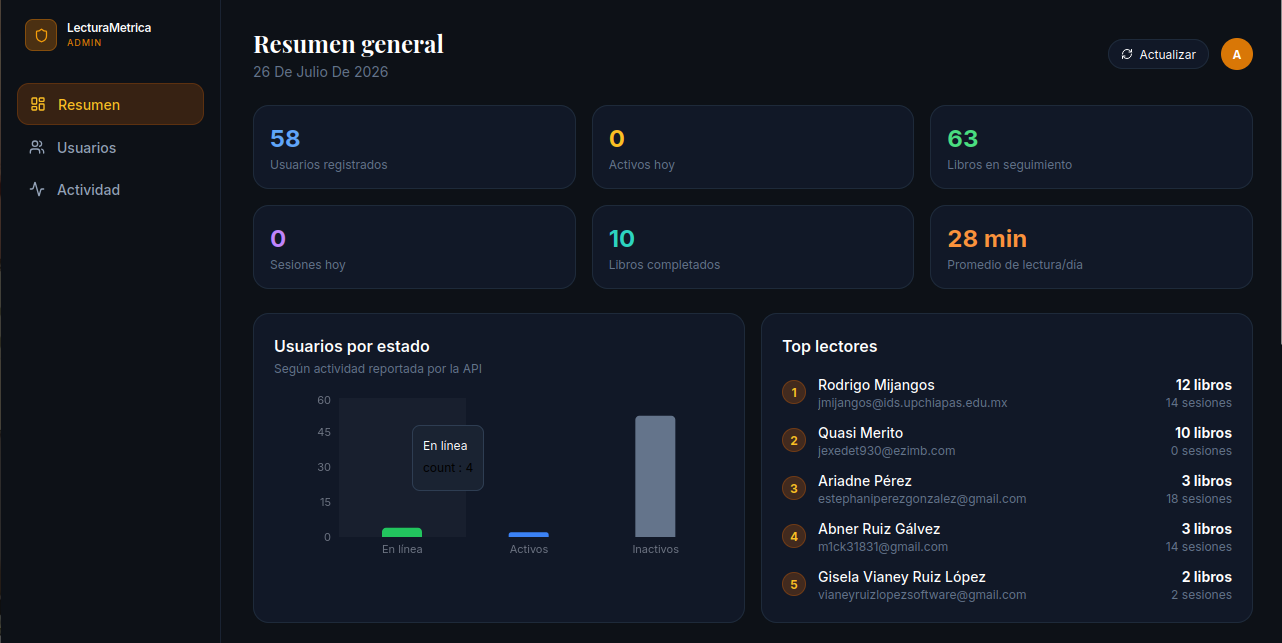
\includegraphics[width=0.85\textwidth]{./fotos/resultados/resumen-26Jul.png} 
    \caption{Panel administrativo mostrando un resumen de actividad.}
    \label{fig:panel_metricas}
\end{figure}

\newpage

% ==============================================================================
% 10. CONCLUSIONES
% ==============================================================================
\section{Conclusiones}

\subsection{Logros alcanzados}
\begin{description}
    \item[\textbf{Arquitectura robusta e integración completa:}] 
    Se construyó una plataforma funcional combinando un \textit{backend} estructurado en Spring Boot con un \textit{frontend} responsivo y moderno en Next.js, logrando comunicaciones eficientes mediante APIs REST desplegadas en entornos de producción.
   
    \item[\textbf{Consolidación de métricas y gamificación:}] 
    Se implementó con éxito un motor de estadísticas en tiempo real capaz de procesar rachas de lectura, metas anuales, registros semanales e insignias dinámicas dentro del perfil del usuario.
\end{description}

\subsection{Lecciones aprendidas}
\begin{description}
    \item[\textbf{Modelado de dominio flexible:}] 
    Diseñar una base de datos preparada para manejar múltiples tipos de obras desde las etapas iniciales evitó refactorizaciones complejas al integrar mangas y \textit{webtoons} junto con libros convencionales.
   
    \item[\textbf{Diseño orientado al \textit{feedback} del usuario:}] 
    Las pruebas con usuarios reales demostraron que restricciones operativas muy rígidas pueden limitar la interacción fluida con la plataforma.
   
    \item[\textbf{Optimización de despliegues en la nube:}] 
    Configurar correctamente los entornos de ejecución en servicios de la nube (como Railway y Supabase) permitió identificar rápidamente cuellos de botella en peticiones HTTP e integrar eficientemente servicios de terceros para el manejo de archivos multimedia.
\end{description}

\subsection{Integración de Inteligencia Artificial en el Desarrollo}
Como parte de las lecciones de desarrollo moderno, el proyecto se apoyó en herramientas de Inteligencia Artificial para mejorar la calidad y eficiencia del código. Cabe destacar que el código fue revisado, ajustado y validado por el equipo de desarrollo en cada iteración; las herramientas de IA funcionaron como asistentes, no como reemplazos del criterio del desarrollador.

\subsubsection*{Aplicación en el Backend (Gemini Pro)}
La integración directa de Gemini Pro en el flujo de trabajo del \textit{backend} abarcó las siguientes áreas:
\begin{itemize}
    \item \textbf{Lógica de Negocio:} Asistencia en el análisis, diseño y estructuración de la lógica interna para módulos complejos, específicamente en el sistema de gamificación (asignación de insignias), el cálculo del seguimiento de rachas de lectura (\textit{streaks}) y el uso de la API externa de Open Library.
    \item \textbf{Estandarización de DTOs:} Redacción y revisión de los mensajes de validación y respuesta dentro de los \textit{Data Transfer Objects} (DTOs), asegurando que la comunicación de la API (mensajes de error, éxito y validaciones) mantenga un tono uniforme, claro y profesional.
    \item \textbf{Optimización de Procesos:} Apoyo en el análisis de código para la refactorización de métodos, simplificación de algoritmos y mejora general del rendimiento dentro de los servicios de la aplicación.
\end{itemize}

\subsubsection*{Aplicación en el Frontend (ChatGPT y Gemini)}
El desarrollo de las interfaces de usuario contó con el apoyo de las siguientes herramientas:
\begin{itemize}
    \item \textbf{ChatGPT (OpenAI):} Resolución de errores de TypeScript en componentes, consultas sobre el comportamiento de \textit{hooks} de React y apoyo en decisiones de la estructura de carpetas del \textit{frontend}.
    \item \textbf{Gemini Pro (Google):} Apoyo en búsquedas de documentación técnica y optimización del código del cliente para un renderizado más eficiente.
\end{itemize}

\subsection{Impacto y reflexión final}
El proyecto demuestra cómo el uso estratégico de la tecnología, las métricas visuales y la gamificación puede transformar una actividad tradicionalmente solitaria en un hábito constante, interactivo y motivador.

LecturaMétrica cobra relevancia al llenar el vacío existente entre los gestores de lectura tradicionales (pensados para libros en formato físico) y la realidad de los lectores modernos, quienes consumen contenido digital en formatos variados. Al combinar el seguimiento de hábitos con dinámicas comunitarias anónimas y la proyección a futuro de espacios de discusión directa, el sistema se posiciona no solo como una herramienta de registro, sino como una plataforma integral para el fomento de la lectura.

Asimismo, al evaluar el impacto y la usabilidad del sistema mediante la recolección de datos cuantitativos de los usuarios reales, se obtuvieron métricas clave sobre la adopción y la retención activa. Como se aprecia en la Figura~\ref{fig:panel_usuarios}, aunque se concretó un registro inicial de usuarios, el análisis del comportamiento reflejó el desafío inherente a la consolidación de hábitos digitales: una notable disminución en la constancia diaria tras los primeros días de uso. Específicamente, del total de usuarios que interactuaron con la plataforma, un sector menor logró mantenerse activo a largo plazo, destacando que únicamente \textbf{2 usuarios} consiguieron superar el umbral de los 10 días de racha continua de lectura. 

Estos resultados empíricos, lejos de representar una limitante técnica, cumplen con el objetivo de evaluación cuantitativa al aportar datos reales sobre el comportamiento del usuario. Esto valida el correcto funcionamiento de los módulos de seguimiento y provee una base analítica fundamental para ajustar las estrategias de retención en futuras versiones del sistema.

\begin{figure}[H]
    \centering
    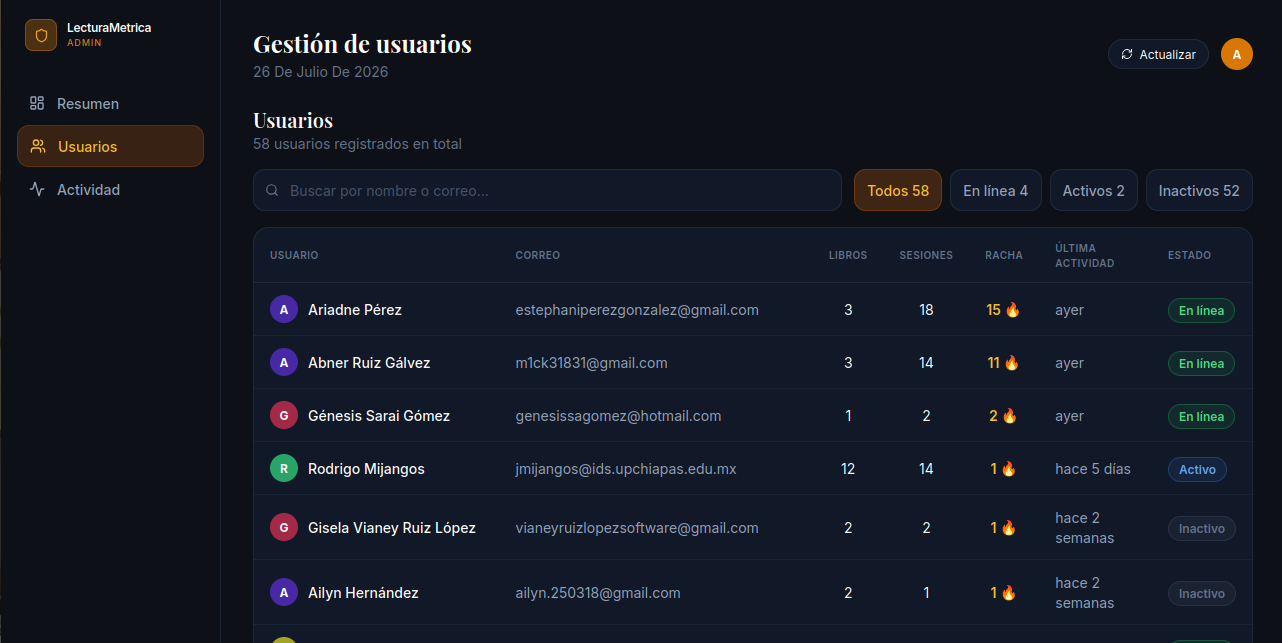
\includegraphics[width=0.85\textwidth]{./fotos/resultados/gestion-26Julio.png} 
    \caption{Actividad y métricas de retención de los usuarios en la plataforma.}
    \label{fig:panel_usuarios}
\end{figure}

\subsection{Diseño visual y optimización de recursos gráficos}
Durante el desarrollo del \textit{frontend}, uno de los aspectos clave abordados fue la identidad visual y el rendimiento de la interfaz orientada a la gamificación. Para garantizar una experiencia de usuario fluida y coherente, se implementaron las siguientes estrategias de diseño y optimización:

\begin{itemize}
    \item \textbf{Consistencia en avatares:} Se diseñó cada avatar bajo un estilo ilustrado unificado (empleando el mismo tipo de trazo, paleta de colores y proporciones), asegurando que todos los elementos pertenezcan a un set visual armónico y no a piezas aisladas.
    \item \textbf{Insignias intuitivas:} Cada insignia fue conceptualizada para representar visualmente el logro desbloqueado (por ejemplo, una llama para las rachas de lectura, una luna para el lector nocturno o un buzón para la interacción comunitaria), permitiendo que el usuario comprenda el significado del incentivo de manera inmediata con solo visualizarlo.
    \item \textbf{Optimización de recursos en formato SVG:} Todos los elementos gráficos principales se implementaron como vectores SVG (con un peso estimado entre $2$ y $3$ KB por archivo). Esto garantizó una nitidez impecable ante cualquier tamaño o densidad de pantalla, evitando el uso de mapas de bits pesados y manteniendo un rendimiento óptimo en la carga de la aplicación.
    \end{itemize}

\newpage

% ==============================================================================
% 11. RECOMENDACIONES
% ==============================================================================
\section{Recomendaciones}
Con la finalidad de dar continuidad al proyecto y potenciar el impacto de la plataforma a futuro, se sugieren las siguientes propuestas de mejora tecnológica y funcional:

\begin{itemize}
    \item \textbf{Módulo de Notificaciones y Recordatorios Automatizados:} Implementar un sistema de notificaciones push enfocado en la retención del usuario, enviando alertas periódicas que incentiven la continuidad del hábito (ej. ``¡No pierdas tu racha diario!'').
    \item \textbf{Gestión de Listas y Colecciones Personalizadas:} Ampliar la flexibilidad de la biblioteca personal mediante la creación de listas temáticas organizadas por el usuario, con la posibilidad de con la comunidad.
    \item \textbf{Subida y Personalización de Avatares/Fotos de Perfil:} Integrar un servicio de almacenamiento de objetos (como Amazon S3) para gestionar la carga y procesamiento de imágenes de perfil personalizadas, reforzando la identidad digital de cada lector.
    \item \textbf{Salas de Chat y Espacios de Discusión Dinámicos:} Incorporar salas de conversación síncronas o foros temáticos para enriquecer el flujo social de la plataforma y fomentar debates sobre lecturas compartidas.
    \item \textbf{Ampliación de Frecuencia en el Buzón de Lectura:} Permitir el envío y recepción de múltiples micro-reseñas o cartas diarias en el ``Buzón del Lector'', flexibilizando los ciclos actuales de 24 horas sin perder la esencia asíncrona y anónima del módulo.
    \item \textbf{Módulo de Moderación y Reporte de Contenido Malicioso:} Desarrollar un mecanismo de control y reporte a nivel de \textit{backend} para prevenir y gestionar conductas maliciosas, permitiendo la detección, moderación o eliminación oportuna de reseñas ofensivas, registros de libros con contenido inapropiado o usuarios infractores que puedan alterar la seguridad y convivencia de la comunidad.
\end{itemize}

\newpage

% ==============================================================================
% REFERENCIAS Y ANEXOS
% ==============================================================================
\begin{thebibliography}{15}

\bibitem{lfpdppp}
Cámara de Diputados del H. Congreso de la Unión. (2010). \textit{Ley Federal de Protección de Datos Personales en Posesión de los Particulares} (LFPDPPP). Texto vigente. \url{http://www.diputados.gob.mx/LeyesBiblio/pdf/LFPDPPP.pdf}

\bibitem{lfda2026}
Cámara de Diputados del H. Congreso de la Unión. (2020). \textit{Ley Federal del Derecho de Autor} (LFDA). Texto vigente. \url{http://www.diputados.gob.mx/LeyesBiblio/pdf/LFDA.pdf}

\bibitem{chiapas2017}
Congreso del Estado de Chiapas. (2017). \textit{Ley de Protección de Datos Personales en Posesión de Sujetos Obligados del Estado de Chiapas}. Periódico Oficial del Estado. \url{https://www.asechiapas.gob.mx/download/leyes/LEY_PROTECCION_DATOS_PERSONALES.pdf}

\bibitem{lfda2026_oficial}
Ley Federal del Derecho de Autor. (2026). \textit{Diario Oficial de la Federación}. Última reforma publicada el 14 de mayo de 2026. \url{http://www.diputados.gob.mx/LeyesBiblio/pdf/LFDA.pdf}

\bibitem{sommerville2016}
Sommerville, I. (2016). \textit{Ingeniería de software} (10a ed.). Pearson.

\bibitem{martin2018}
Martin, R. C. (2018). \textit{Clean Architecture: A Craftsman's Guide to Software Structure and Design}. Prentice Hall.

\bibitem{spring2025}
Spring Framework Team. (2025). \textit{Spring Boot Reference Documentation}. Core Software Press. \url{https://spring.io/projects/spring-boot}

\bibitem{nextjs2025}
Vercel. (2025). \textit{Next.js Documentation: Building Your Application}. Vercel Inc. \url{https://nextjs.docs/docs}

\bibitem{postgres2025}
The PostgreSQL Global Development Group. (2025). \textit{PostgreSQL 16 Official Documentation}. \url{https://www.postgresql.org/docs/16/index.html}

\bibitem{inegi2025}
Instituto Nacional de Estadística y Geografía (INEGI). (2025). \textit{Módulo sobre Lectura (MOLEC)}. \url{https://share.google/oSIT0jhQy8hLjdmqe}

\bibitem{dialnet2024}
Dialnet. (2024). \textit{Factores que afectan el hábito de la lectura: un problema de la sociedad actual}. \url{https://share.google/RAG5lluZnsl7iiICb}

\bibitem{ocnos2009}
Revista OCNOS. (2009). \textit{Aunque lea poco, yo sé que estoy listo}. \url{https://share.google/1MDzQisS2FaRMtEf9}

\bibitem{eciencias2020}
E-Ciencias de la Información. (2020). \textit{Hábitos de lectura en alumnos de primer ingreso de psicología educativa de la Universidad Pedagógica Nacional (UPN), México}. Vol. 10, N° 1. \url{https://www.scielo.sa.cr/scielo.php?script=sci_arttext&pid=S1659-41422020000100231}

\bibitem{ride2025}
RIDE. Revista Iberoamericana para la Investigación y Desarrollo Educativo. (2025). \textit{Las creencias de estudiantes de secundaria sobre la lectura}. Vol. 15, N° 30. \url{https://www.scielo.org.mx/scielo.php?script=sci_arttext&pid=S2007-74672025000100135}

\end{thebibliography}

\subsection{Anexos}

\begin{figure}[H]
    \centering
    
\includegraphics[width=0.85\textwidth]{/home/minchito/Escritorio/LM_PI_salvavidas/latex/fotos/sirgei/login.jpeg}
    \caption{Interfaz del formulario de inicio de sesión.}
    \label{fig:login}
\end{figure}

\begin{figure}[H]
    \centering
    
\includegraphics[width=0.85\textwidth]{/home/minchito/Escritorio/LM_PI_salvavidas/latex/fotos/sirgei/2fa.jpeg}
    \caption{Pantalla de verificación de autenticación de dos factores (2FA).}
    \label{fig:2fa}
\end{figure}

\begin{figure}[H]
    \centering
    
\includegraphics[width=0.85\textwidth]{/home/minchito/Escritorio/LM_PI_salvavidas/latex/fotos/sirgei/2fa-2.jpeg}
    \caption{Configuración y adición de nuevo método 2FA.}
    \label{fig:add_2fa}
\end{figure}

\begin{figure}[H]
    \centering
    
\includegraphics[width=0.85\textwidth]{/home/minchito/Escritorio/LM_PI_salvavidas/latex/fotos/sirgei/entrar.jpeg}
    \caption{Confirmación de acceso al sistema.}
    \label{fig:entrar}
\end{figure}

\begin{figure}[H]
    \centering
    
\includegraphics[width=0.85\textwidth]{/home/minchito/Escritorio/LM_PI_salvavidas/latex/fotos/sirgei/login-postman.png}
    \caption{Prueba de la API de inicio de sesión realizada en Postman.}
    \label{fig:login_postman}
\end{figure}

\begin{figure}[H]
    \centering
    
\includegraphics[width=0.85\textwidth]{/home/minchito/Escritorio/LM_PI_salvavidas/latex/fotos/sirgei/2fa-postman.png}
    \caption{Prueba de la API en la verifiación de dos pasos.}
    \label{fig:jmeter_simultaneo_fallido}
\end{figure}

\begin{figure}[H]
    \centering
    
\includegraphics[width=0.85\textwidth]{/home/minchito/Escritorio/LM_PI_salvavidas/latex/fotos/sirgei/summary-report.png}
    \caption{Jmeter resumen de un reporte.}
    \label{fig:jmeter_simultaneo}
\end{figure}

\begin{figure}[H]
    \centering
    
\includegraphics[width=0.85\textwidth]{/home/minchito/Escritorio/LM_PI_salvavidas/latex/fotos/sirgei/view-result-fallido.png}
    \caption{Jmeter resultados exito y fallo.}
    \label{fig:jmeter_simultaneo}
\end{figure}

\subsection*{Anexo A: Manual de Usuario}
\addcontentsline{toc}{subsection}{Anexo A: Manual de Usuario}
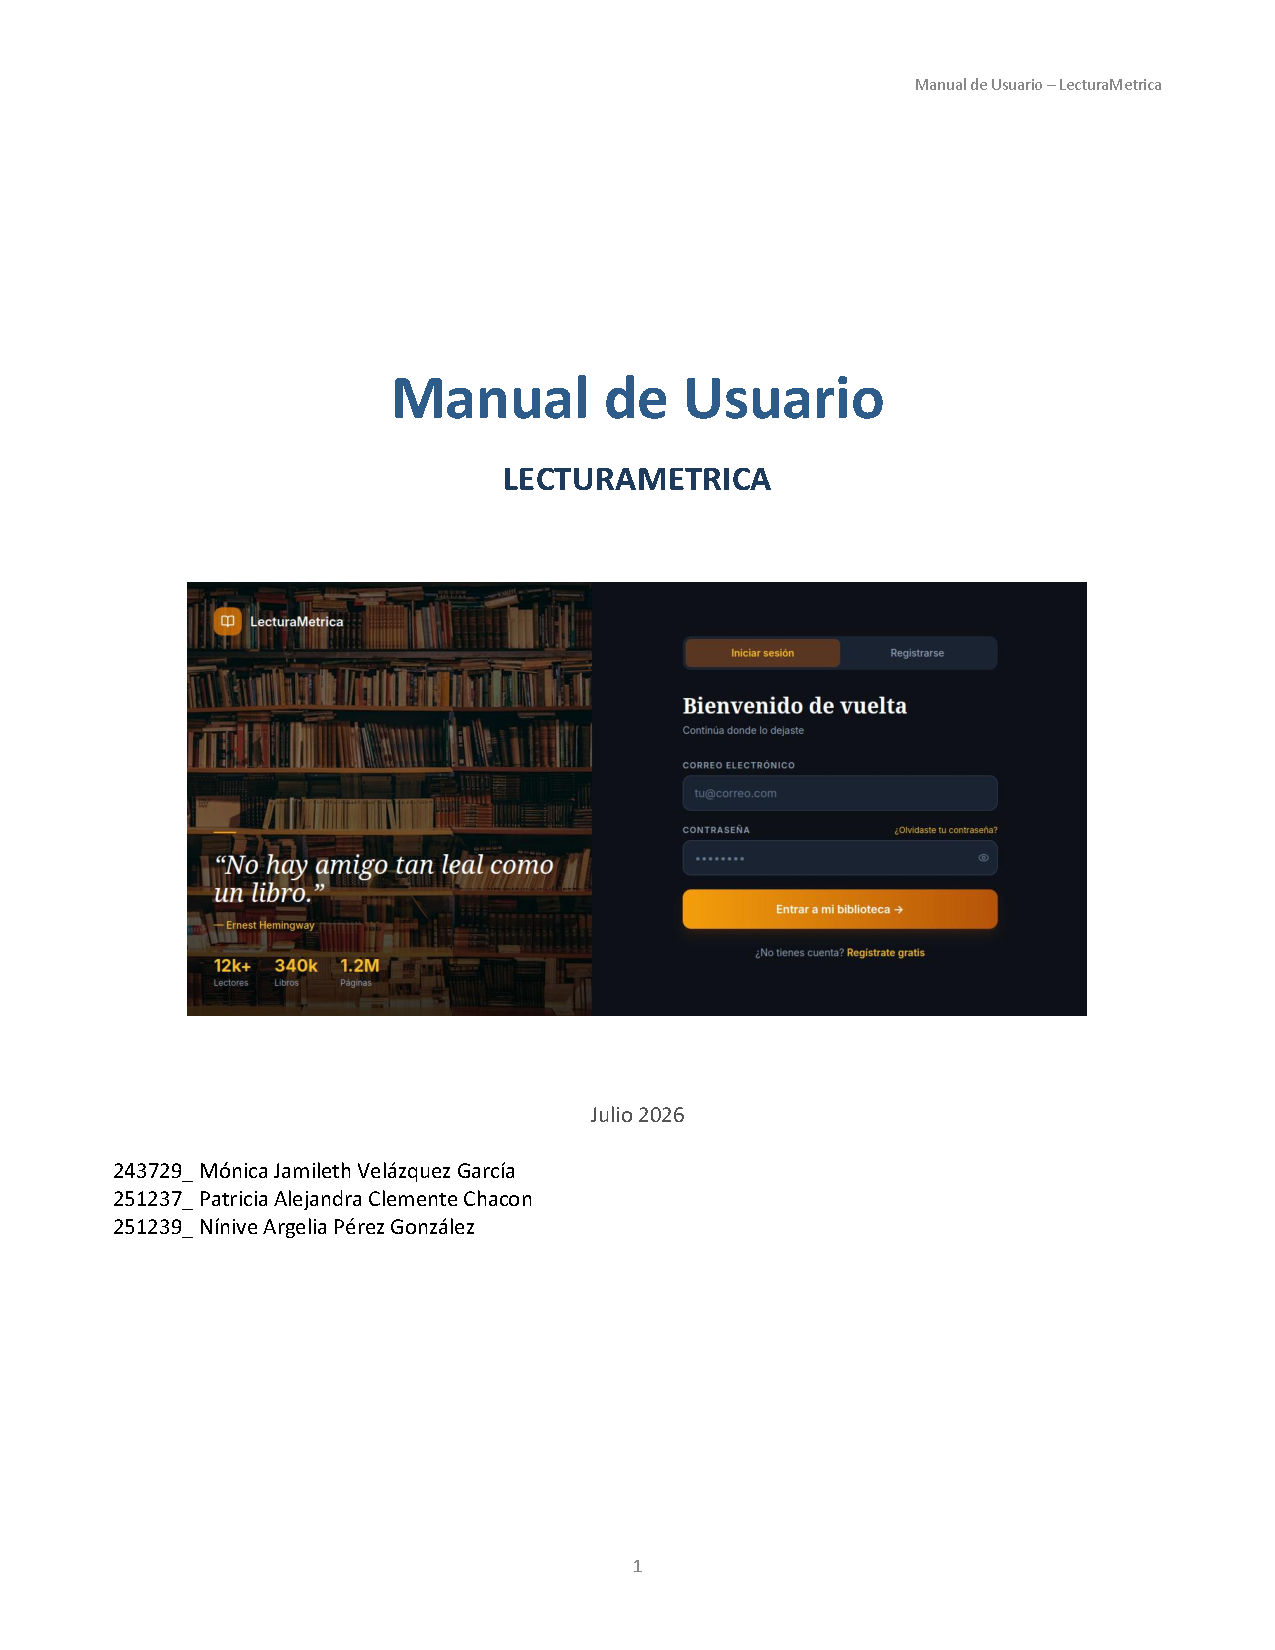
\includepdf[pages=-]{./anexos/Manual_de_Usuario.pdf}

\end{document}